%===================================== CHAP 3 =================================

\chapter{Design}

A Leslie Rotating speaker is not a high-fidelity speaker, it is not meant to have the flattest possible frequency response. A Leslie speaker is used to change the sound, not reproduce it \citep{TheatreOrgansMysteryLeslie}.

This chapter presents the current design, which builds on and revises the prototype from the preceding specialisation project \citep{horpedal2025projectthesis}. Many intermediate iterations are omitted; only the key alternatives are discussed at the relevant decision points, with remaining limitations revisited in the discussion.

\section{Electronics}

\subsection{Moteus C1 motor controller}
The motor controller chosen for this project is the Moteus C1 motor controller. It turns a hobby brushless motor into a high-performance servo-actuator for low-cost and low-power systems \textbf{TODO: kilde, mjbots.com}. It is an open source project and features
\begin{itemize}
	\item Field Oriented Control
	\item An integrated magnetic encoder
	\item High-speed CAN-fd communication at 5Mbps
	\item Position, velocity, and torque control with acceleration and velocity limited trajectories
	\item Fast control loops running at 15-30kHz.
\end{itemize}

%(kilde https://mjbots.github.io/moteus/)

\subsection{Observing the load with ma600 magnetic encoder}

\subsection{Arduino Nano Esp32}

\subsection{CAN Breakout board}
In order for the Arduino Nano ESP32 to communicate with the moteus c1 motor controller with CAN fd, a CAN-fd transceiver and receiver is needed. The CAN Transceiver MCP2518 from Soldered Electronics features a MCP2518FD IC that allows the use of both CAN 2.0B and CAN-fd \textbf{TODO: kilde datablad}. It also features an on-board jumper to activate a 120 Ohm termination resistor. It is similar to the moteus C1 motorcontroller an open source project. The GitHub repository contains both 3D step files and schematics (see \autoref{app:mcp2518}) which eases integration with other components. The Arduino Nano Esp32 connects to CAN breakout board via SPI, the schematic is seen in fig x.

\begin{figure}
	\begin{center}
		\includesvg[width=0.3\textwidth]{fig/design/Arduino-nano-and-can-breakout.svg}
	\end{center}
	\caption{}\label{fig:arduino-nano-can-breakout}
\end{figure}


The Schematic of the CAN bus is presented in fig y.
\citep{soldered_mcp2518_overview}

\subsection{Resistor Ladder for input selection}


\subsection{Choice of bottom woofer/speaker}
\textbf{TODO: justify the choice of speakers EV1824M Celestion}

\subsection{Choice of horn driver}
The original horn driver used in the Leslie 122 is the Jensen V21 \textbf{TODO: legg inn kilde}. A frequency response curve of this particular
speaker was not retrievable. However studying vendors selling replacement horn drivers it is possible to infer the preferred frequency
range.

The Electro Voice 1825M was bought from finn.no for 600 kr. According to its datasheet (see \autoref{app:EV1824M}) it delivers
plus minus 5 dB between 300 to 4500 Hz.

\subsection{Crossover network}
In classic Leslie speakers like the Leslie 122, a crossover network splits the audio signal from the amplifier with bass going to the bottom woofer and treble to the upper horn driver. The filter is a 2nd order Butterworth filter with the crossover placed at 800Hz \textbf{TODO: sett inn kilde}.

However since this Leslie build is more aimed at being used with guitar and organ a little less bass is needed since the guitar doesn't have as much bass frequency as an Organ.

The following crossover was designed based on parts earlier acquired.

\begin{figure}[H]
	\centering
	\begin{circuitikz}[american]
    \node[left] at (0,6) {Amp.\,In$+$};
    \node[left] at (0,0) {Amp.\,In$-$};

    % Input wire to split junction
    \draw (0,6) to[short, o-] (2,6) node[circ] {};

    % C1 in the horizontal lead (horn series capacitor)
    \draw (2,6) to[C, l=$C_1{=}18\;\mathrm{\mu F}$] (7,6) node[circ] {};

    % Woofer branch: L1 in series, then woofer straight down to ground
    \draw (2,6) to[L, l=$L_1{=}1.6\;\mathrm{mH}$] (2,3.5);
    \draw (2,3.5) to[loudspeaker, l=Woofer] (2,1);
    \draw (2,1) -- (2,0);
    \node[circ] at (2,0) {};

    % L2 shunt from horn junction down to ground
    \draw (7,6) to[L, l_=$L_2{=}1.6\;\mathrm{mH}$] (7,0);
    \node[circ] at (7,0) {};

    % Horn driver: short wire right from junction, then down to ground
    \draw (7,6) -- (8,6);
    \draw (8,6) to[loudspeaker, l=Horn] (8,1);
    \draw (8,1) -- (8,0);
    \node[circ] at (8,0) {};

    % Ground rail
    \draw (0,0) to[short, o-] (9,0);
\end{circuitikz}

	\caption{Passive crossover network. $L_1$ forms a low-pass section routing low frequencies to the woofer. $C_1$ and shunt $L_2$ form a second-order high-pass section routing high frequencies to the horn driver.}
	\label{fig:crossover}
\end{figure}

For the woofer low-pass section, the series inductor $L_1$ with a nominal speaker impedance of $R = 8\,\Omega$ gives a first-order $-3\,\text{dB}$ cutoff frequency of
\[
	f_L = \frac{R}{2\pi L_1} = \frac{8}{2\pi \times 1.6 \times 10^{-3}} \approx 796\,\text{Hz}
\]
For the horn high-pass section, $C_1$ and $L_2$ form an $LC$ network whose natural frequency is
\[
	f_H = \frac{1}{2\pi\sqrt{L_2 C_1}} = \frac{1}{2\pi\sqrt{1.6\times10^{-3} \times 18\times10^{-6}}} \approx 938\,\text{Hz}
\]

\citep{dickason_loudspeaker_cookbook}. \textbf{[TODO: verifiser kilde.]}

\clearpage
\section{Mechanical}
All parts were designed in Autodesk Fusion with a bottom up approach, meaning the parts are designed individually before being assembled into a complete design. \textbf{TODO: finn kilde, vurder om dette stemmer}


\textbf{TODO: Justify why the rotors are not enclosed to increase the AM-modulation.}

\subsection{Design of Horn}

A picture of a Leslie horn next to a ruler was found on the internet \textbf{TODO: putt inn bilde i vedlegg} with the ruler in the same picture it made it possible to infer some of the dimensions of this horn. The diameter of the throat was approximated to \textbf{TODO: ...} with the use of \textbf{TODO: online tool} and the length of the horn projected down in a xy-plane was approximated to \textbf{TODO: yy}.

This was used as a starting point for the design.

The centre line of the horn was parameterized into a vertical straight section of length $L_1$, a circular-arc bend of radius $R$, and a second straight section of length $L_2$ angled $\alpha$ above the horizontal, see \autoref{fig:horn-centerline}.

\begin{figure}[H]
	\centering
	\begin{tikzpicture}[font=\small, >=stealth, line cap=round]

  % L1 = 1.5, R = 2, arc 180°→110° clockwise, L2 = 3.5
  % O = (2, 1.5),  C = O + 2·(cos110°, sin110°) ≈ (1.316, 3.380)
  % D = C + 3.5·(cos20°, sin20°) ≈ (4.606, 4.577)

  \coordinate (A) at (0,     0    );
  \coordinate (B) at (0,     1.5  );
  \coordinate (O) at (2,     1.5  );
  \coordinate (C) at (1.316, 3.380);
  \coordinate (D) at (4.606, 4.577);

  % centreline
  \draw[very thick] (A) -- (B);
  \draw[very thick] (B) arc[start angle=180, end angle=110, radius=2];
  \draw[very thick] (C) -- (D);

  % travel arrows
  \draw[->, thick, gray!60] (0, 0.50) -- (0, 1.00);
  \draw[->, thick, gray!60] (2.726, 3.893) -- (3.196, 4.064);

  % arc centre + R label (135°)
  \filldraw[gray!60] (O) circle (2pt);
  \draw[gray, dashed] (O) -- (0.586, 2.914) node[midway, left, black] {$R$};

  % L1 dimension
  \draw[gray, dotted] (A) -- (-0.70, 0  );
  \draw[gray, dotted] (B) -- (-0.70, 1.5);
  \draw[<->, gray]    (-0.60, 0) -- (-0.60, 1.5)
      node[midway, left, black] {$L_1$};

  % L2 dimension (perp offset 0.5 in direction (−sin20°, cos20°))
  \draw[gray, dotted] (C) -- (1.145, 3.850);
  \draw[gray, dotted] (D) -- (4.435, 5.047);
  \draw[<->, gray]    (1.145, 3.850) -- (4.435, 5.047)
      node[midway, above left, black] {$L_2$};

  % exit angle α
  \draw[gray, dashed] (C) -- (3.0, 3.380);
  \draw[->, gray] (2.166, 3.380)
      arc[start angle=0, end angle=20, radius=0.85]
      node[pos=0.5, right, black] {$\alpha$};

  % labels
  \node[below]       at (A) {Throat};
  \node[above right] at (D) {Mouth};

\end{tikzpicture}

	\caption{Parametric centreline geometry of the horn. Sound enters at the throat and travels upward along $L_1$, bends through a circular arc of radius $R$, and exits along $L_2$ at angle $\alpha$ above the horizontal.}
	\label{fig:horn-centerline}
\end{figure}


Then AI was used to generate a script generating circles along the centreline with areas corresponding to \textbf{TODO: referer til horn-equation i background}. The circles were then connected with the use of loft in Autodesk Fusion to generate the airway of the horn \textbf{TODO: forklar hva det betyr}.

\begin{figure}[H]
	\begin{center}
		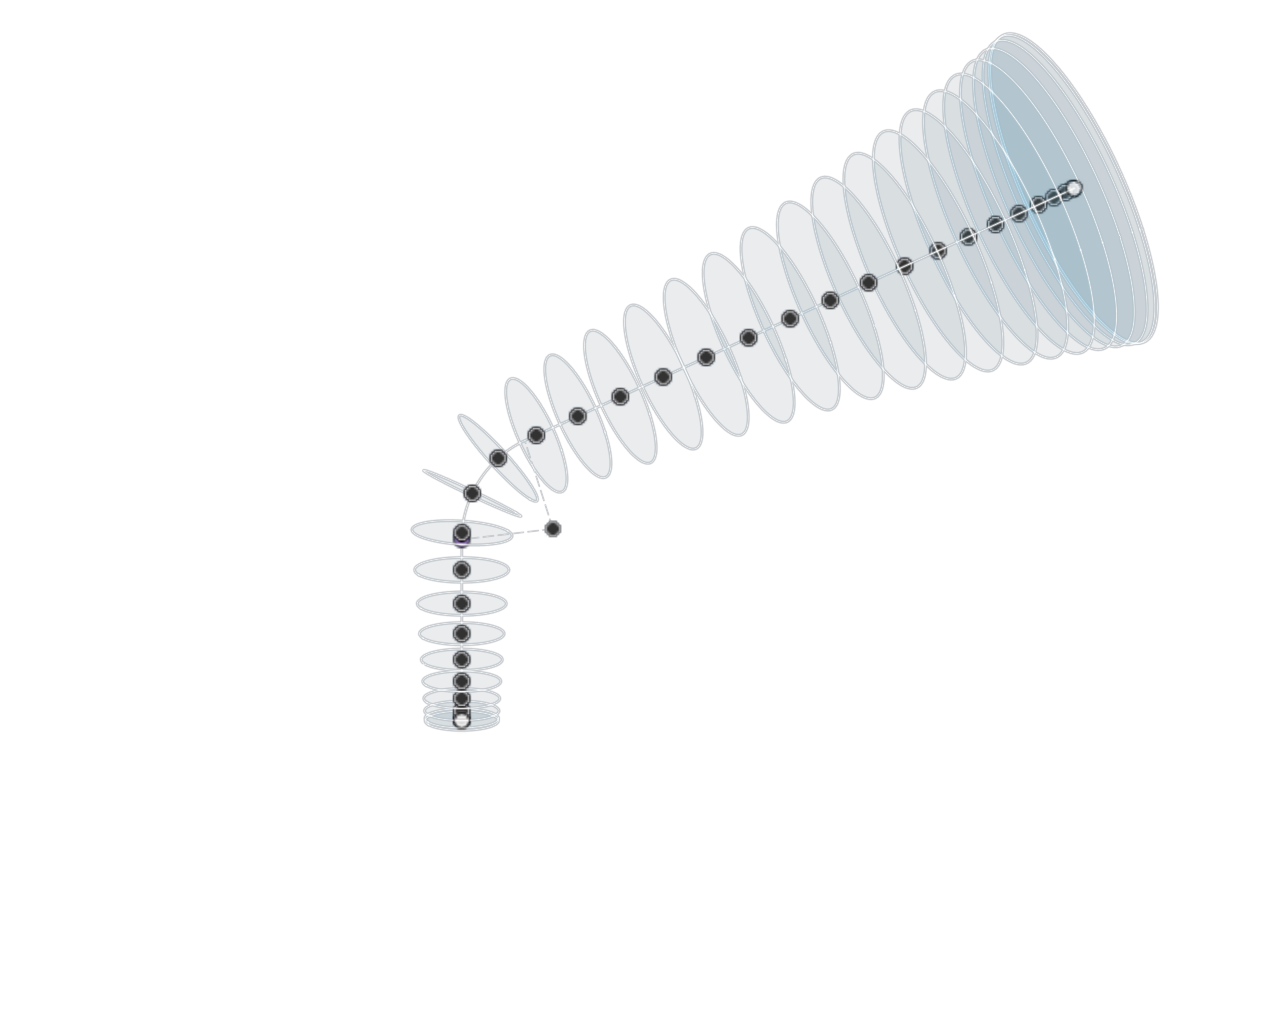
\includegraphics[width=0.48\textwidth]{fig/design/horn-air-way-circles.png}\hfill
		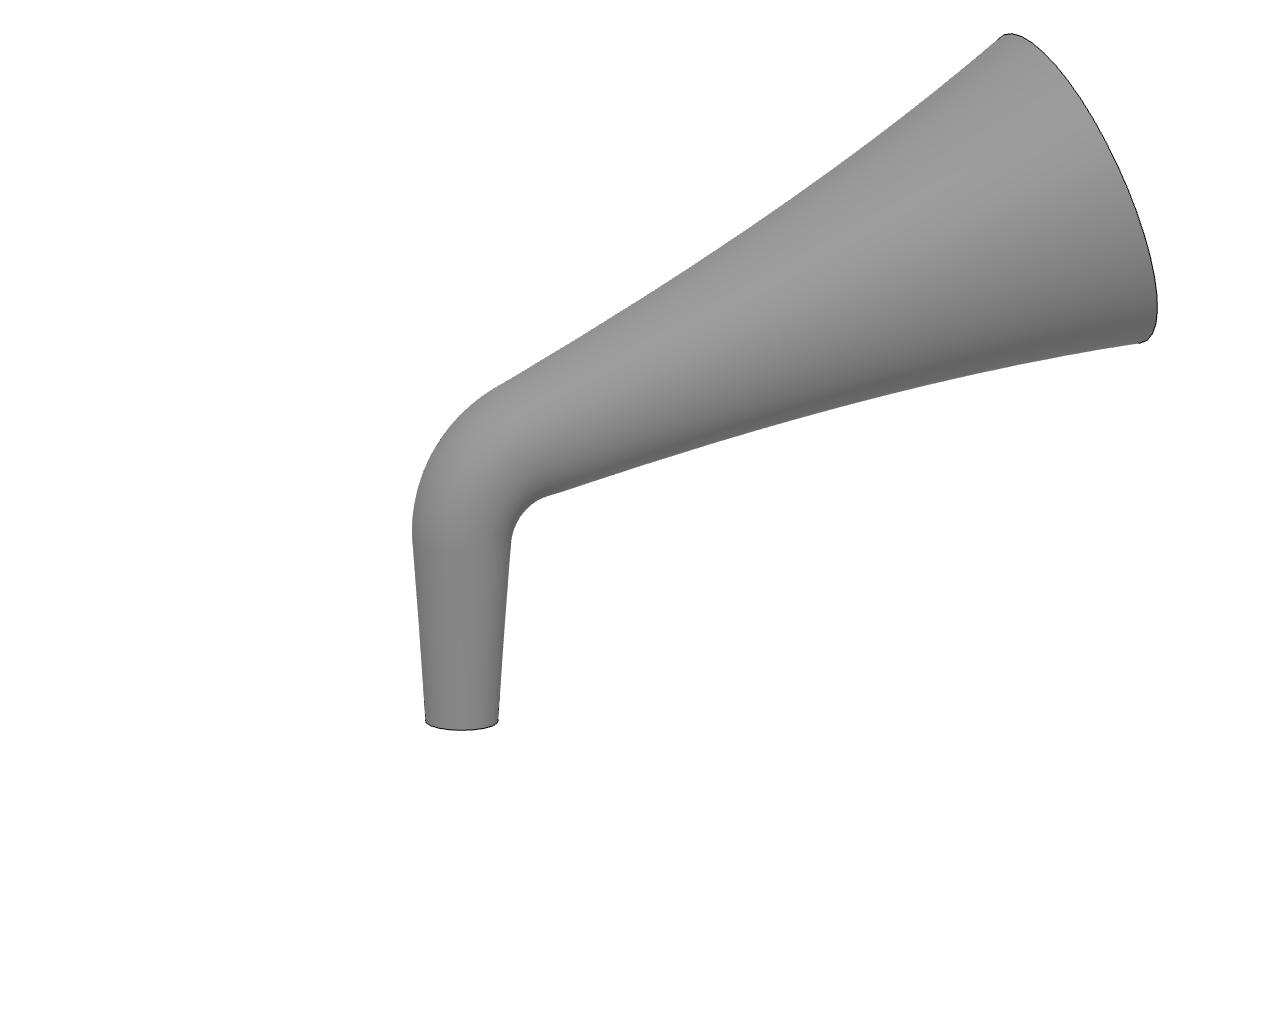
\includegraphics[width=0.48\textwidth]{fig/design/airway-body.png}
	\end{center}
	\caption{}\label{fig:horn-air-way-circles}
\end{figure}


The parameters of \textbf{TODO: blabla} were determined more by practical mechanical constraints \textbf{TODO: the turning radius is way too steep, finn kilde som sier at den skal være x antall større enn diameter}.

To verify the design the equation from background was used. Here it is assumed the horn is straight something it obviously is not \textbf{TODO: si noe om at det er en stor antagelse}.


The flare constant $m$ can be determined from the throat diameter $d_t = 22\,\text{mm}$, mouth diameter $d_m = 101.6\,\text{mm}$, and acoustic centreline length $L = 285\,\text{mm}$. The throat and mouth areas are
\[
	S_0 = \pi\!\left(\frac{d_t}{2}\right)^{\!2} = \pi(0.011)^2 \approx 3.80\times10^{-4}\,\text{m}^2, \qquad
	S_L = \pi\!\left(\frac{d_m}{2}\right)^{\!2} = \pi(0.0508)^2 \approx 8.11\times10^{-3}\,\text{m}^2
\]
From \autoref{eq:horn-area}, the flare constant is
\[
	m = \frac{\ln(S_L/S_0)}{L} = \frac{\ln(21.3)}{0.285} \approx 10.7\,\text{m}^{-1}
\]
Substituting into \autoref{eq:horn-cutoff} gives the cutoff frequency
\[
	f_c = \frac{mc}{4\pi} = \frac{10.7\times 343}{4\pi} \approx 293\,\text{Hz}
\]
This is below the driver's rated lower limit of 300\,Hz, confirming that the horn supports the full operating range of the driver.

The horn itself could then be designed around the airway of the horn, similarly to other Leslies a dummy horn placed on the opposite side was added in order to place the centre of mass on the axis of rotation.

\begin{figure}[H]
	\begin{center}
		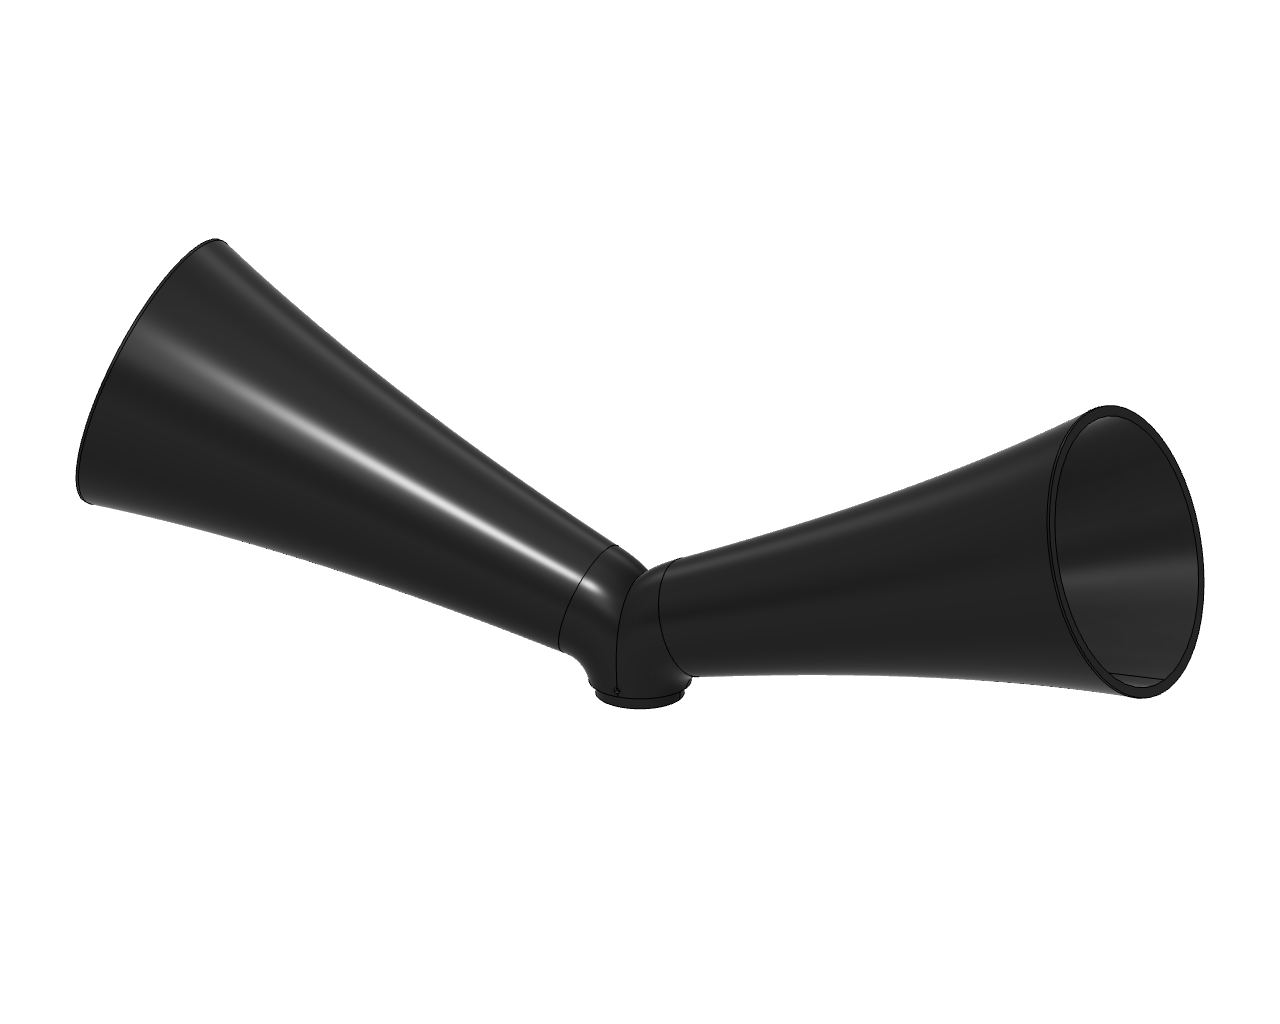
\includegraphics[width=0.48\textwidth]{fig/design/horn.png}\hfill
		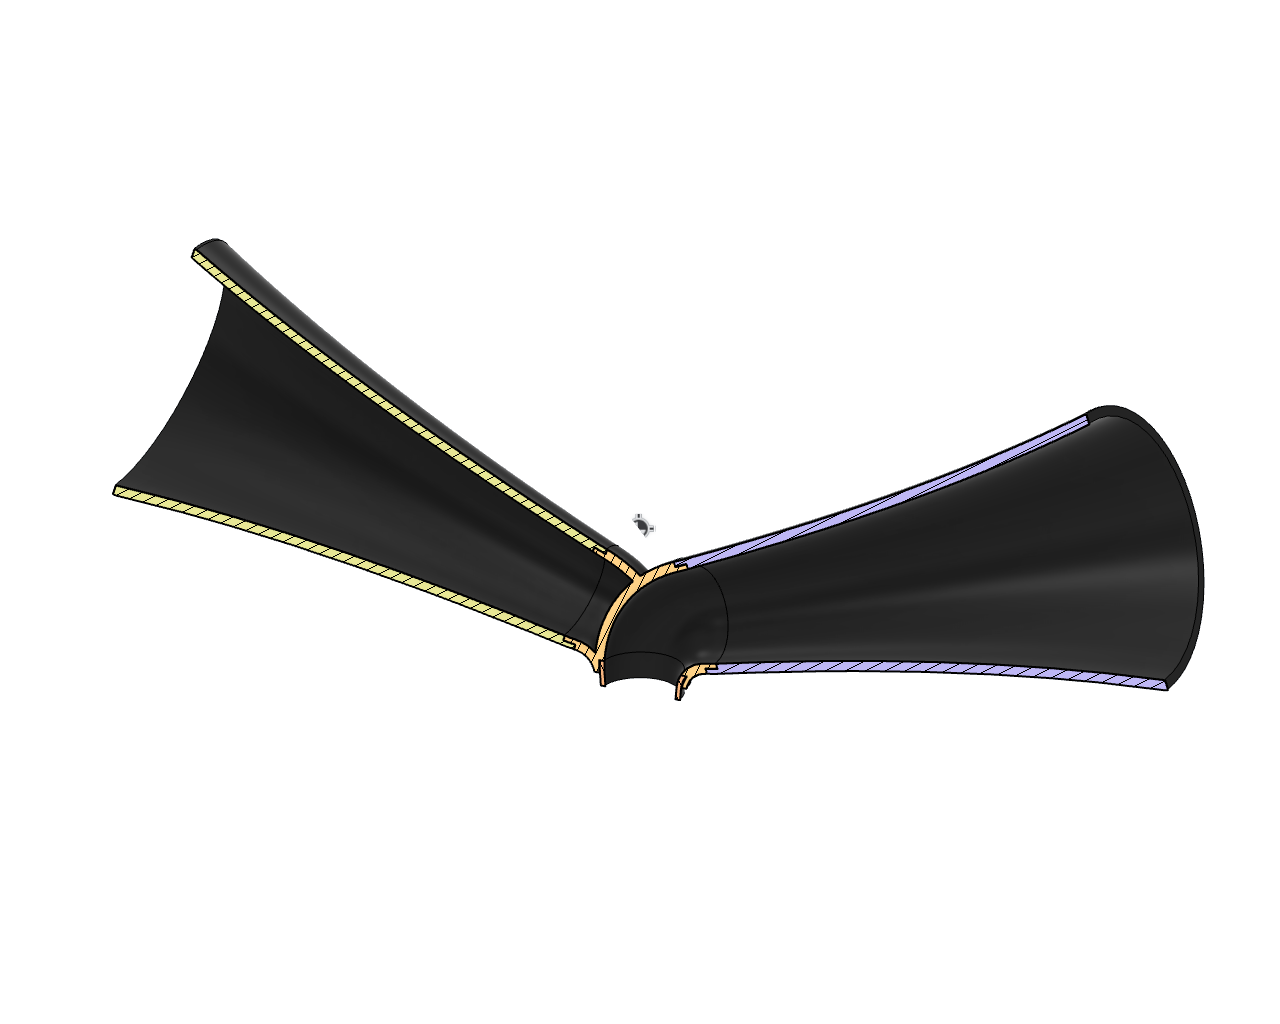
\includegraphics[width=0.48\textwidth]{fig/design/horn cross section.png}
	\end{center}
	\caption{}\label{fig:horn-design}
\end{figure}
\subsection{Design of Drum}
The drum earlier designed and implemented was based on some approximate estimates of the size of the drum of a Leslie \textbf{TODO: specify model}. However since this project will use a 12 inch speaker as the woofer, it is assumed that it is sensible to scale the diameter of the drum to a $\frac{12}{15}$.
The earlier drum also when rotating at the upper end of velocities caused the enclosure to wiggle, indicating a not properly balanced rotor.
To try to overcome this, special caution in the design was taken. With the help of AI tools an add-in for Autodesk Fusion was coded, which can be used to align the principal inertia axis of the drum with the z-axis, ensuring both static balance and dynamic balance \textbf{TODO: finn kilde}.

\textbf{TODO: fant en youtube-video med en som tok mål.}
\begin{figure}[H]
	\begin{center}
		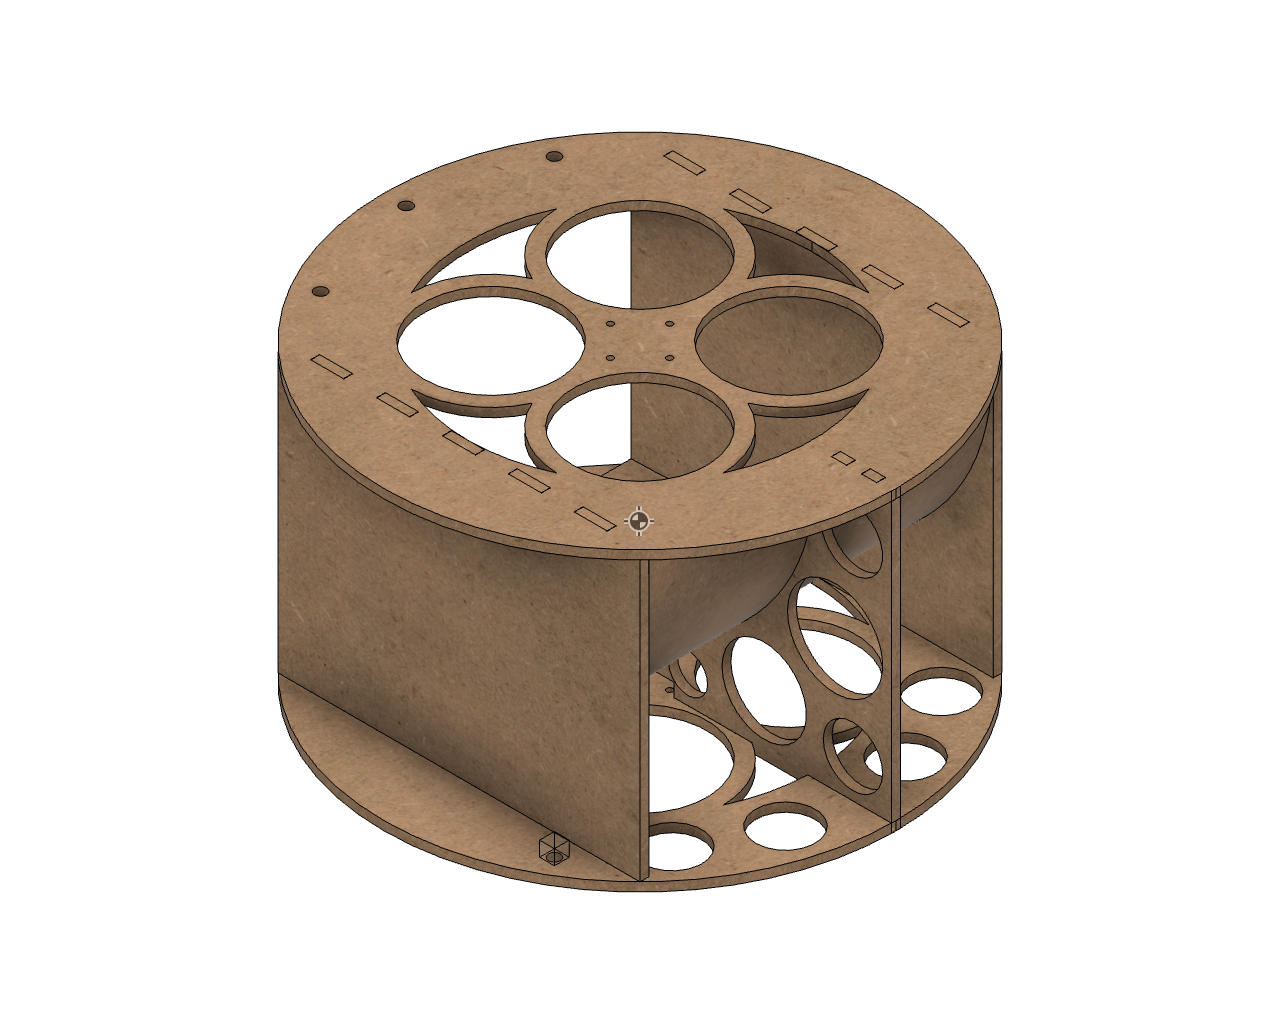
\includegraphics[width=0.48\textwidth]{fig/design/drum-back.png}
		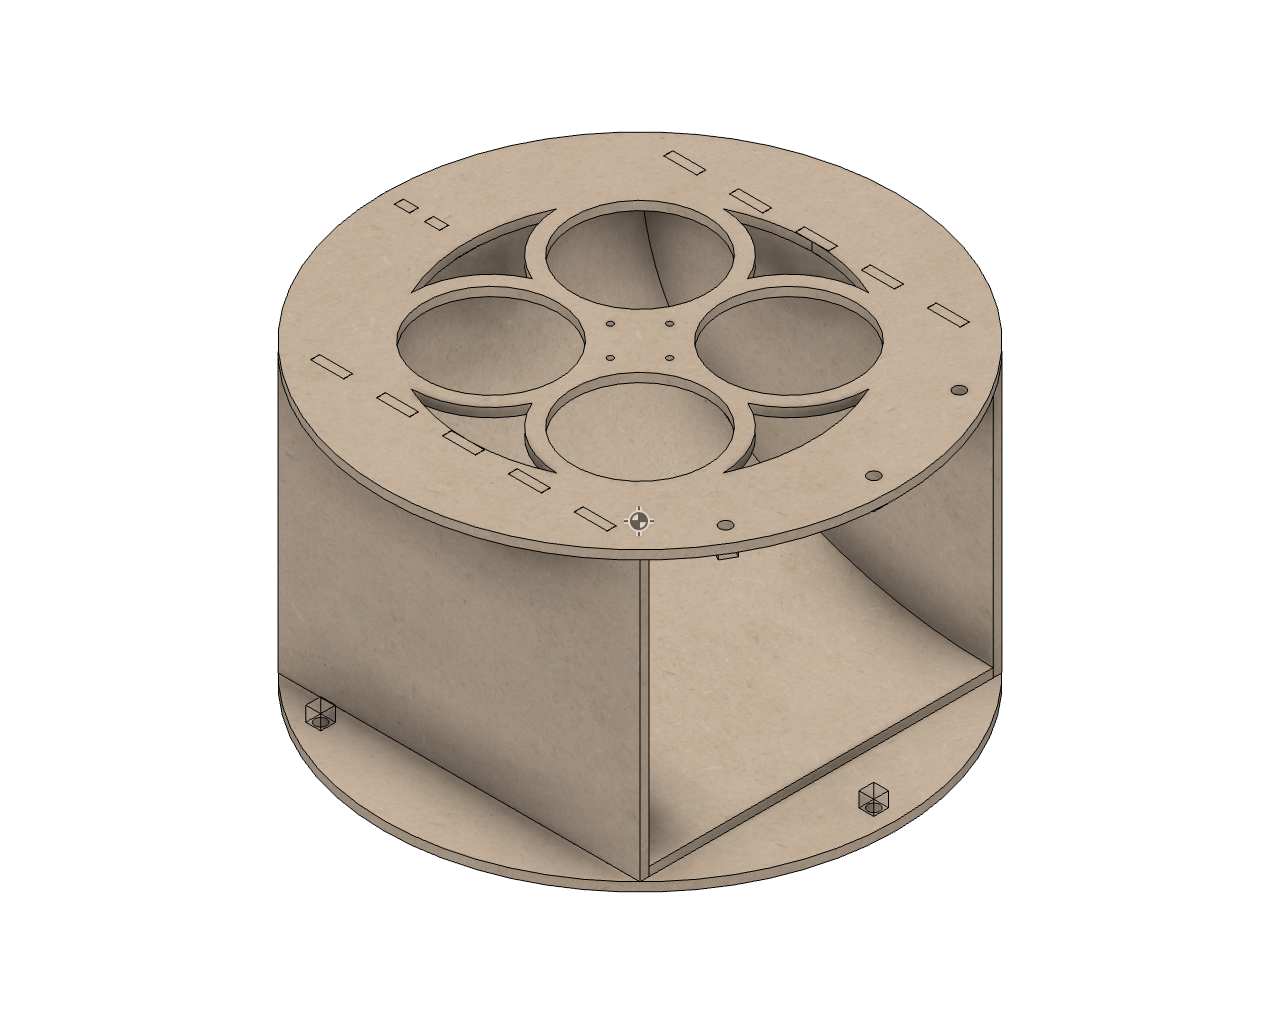
\includegraphics[width=0.48\textwidth]{fig/design/drum-front.png}
	\end{center}
	\caption{}\label{fig:drum-front-back}
\end{figure}

\subsection{Drive belt and pulleys}
Early testing showed that the 6mm drive belt used was a source of mechanical noise and therefore 3mm was used instead.

\textbf{TODO: begrunne hvorfor giring kan være lurt}
The motors are rated for 4000 rpm \textbf{TODO: ref appendix}. Also the motor controller is more aimed at high-speed control \textbf{TODO: sett inn kilde fra moteus}. \textbf{TODO: si noe om torque multiplying.}

Therefore a gearing factor of 3.5 and 4.0 was chosen \textbf{TODO: lag fancy tabell}. The centre to centre distances were decided by practical considerations, with the load placed in the middle of the square of the cabinet and the motor pulley placed with distances to walls in mind. That yielded the centre to centre distances: \textbf{TODO: blablabla}

In previous work the 6mm drive belt had audible noise coming from the drive belt. At this thickness a correct install-tension was too great \textbf{TODO: fortsett å si hvorfor 6mm ikke funka bra}. Therefore it was decided to try to use the 3 mm version instead.

\textbf{TODO: referer til appendix og datasheet} Shows the rated working loads at different install tensions for the 3mm drive belt. A simple calculation for both ends of the scale with some assumptions of mass \textbf{TODO: andre parametere} gives the following achievable acceleration with tensions of 0 to 10 percent.

which shows it is sufficient with proper tension.

The cut length for each belt could then be calculated, following the instructions from the manufacturer \textbf{TODO: ref appendix}. First the reference length is calculated:
\begin{equation}
	L = 2C + \frac{\pi}{2}(D+d) + \frac{(D-d)^2}{4C}
	\label{eq:referece-length}
\end{equation}
This gives reference lengths \textbf{TODO: x and y} for the upper and lower rotors.
\textbf{TODO: appendix} gives the following formula for cut length when a butt weld is done.
\begin{equation}
	Cut Length = \frac{Reference Length}{1 + \% tension}
	\label{eq:cut-length}
\end{equation}

\textbf{TODO: Which becomes x and y for the upper and lower drive system}

\subsection{Assembling pulleys with deflectors}

\begin{figure}
	\begin{center}
		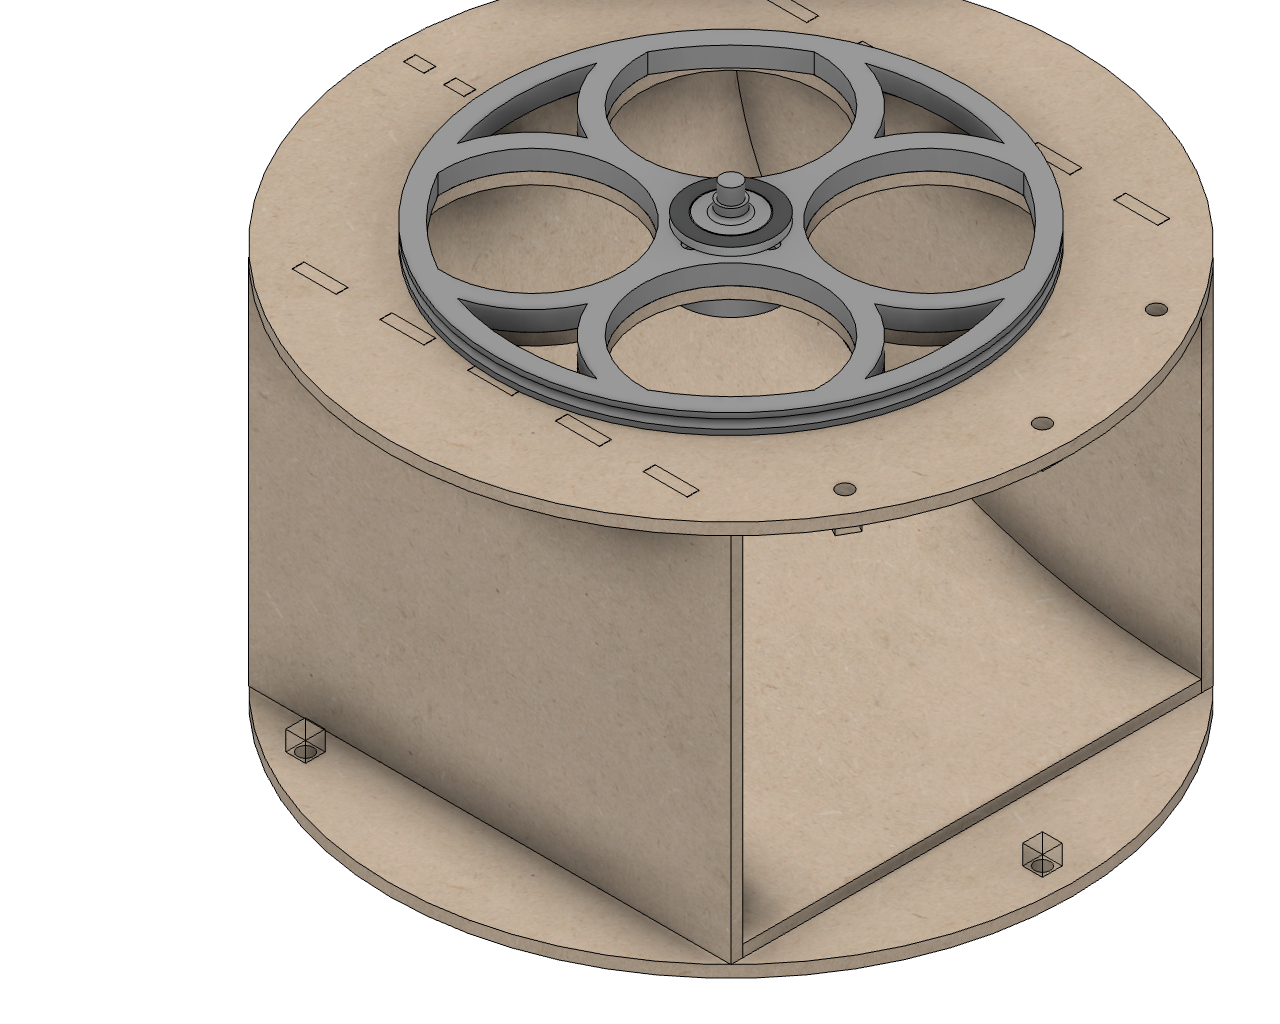
\includegraphics[width=0.48\textwidth]{fig/design/drum-and-pulley.png}
		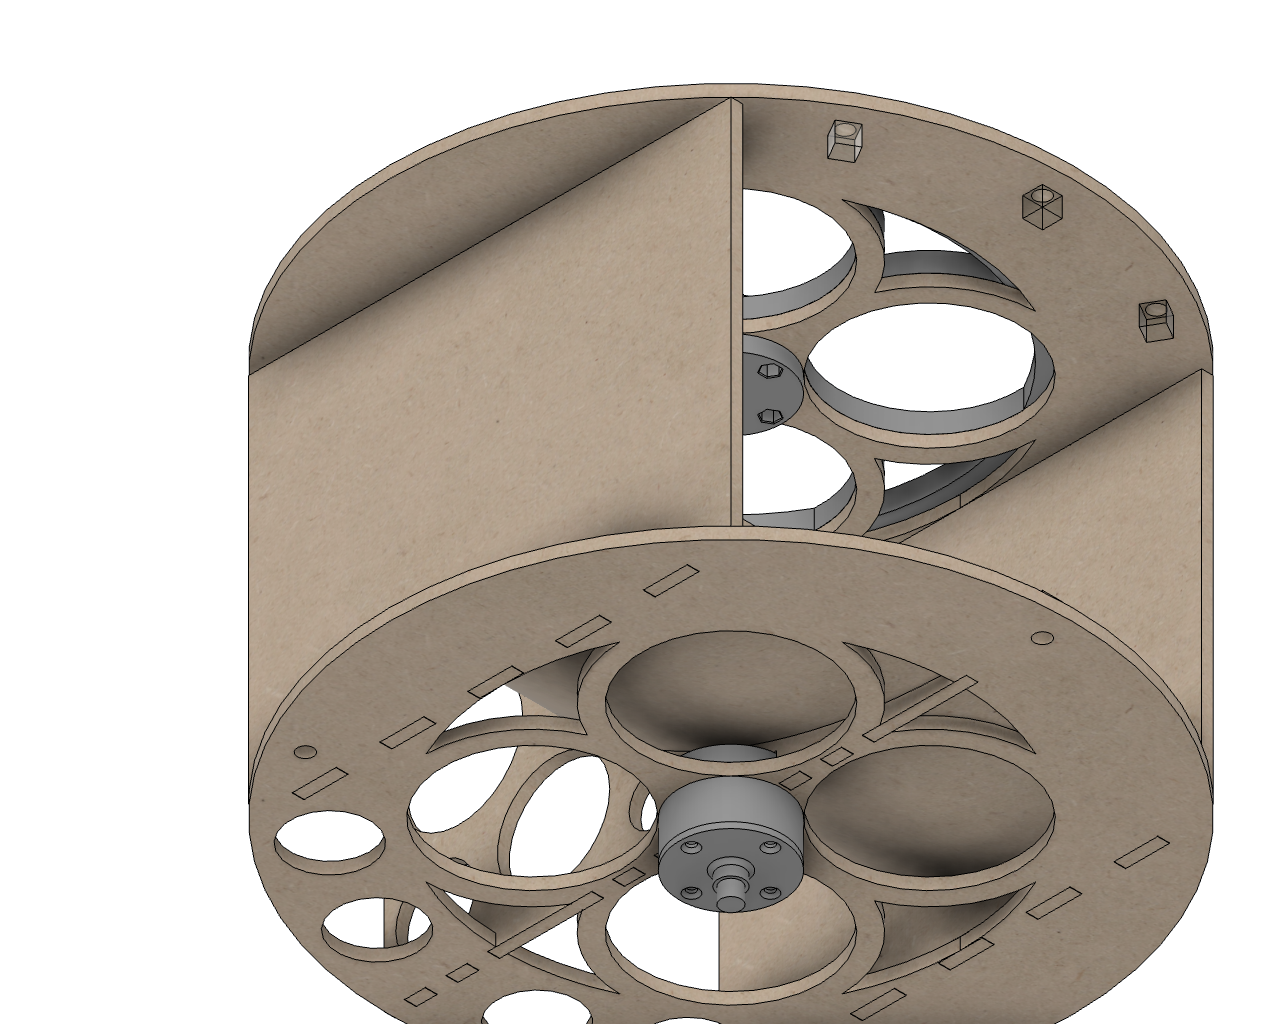
\includegraphics[width=0.48\textwidth]{fig/design/drum-and-pulley-bottom.png}
	\end{center}
	\caption{}\label{fig:drum-and-pulley}
\end{figure}

\begin{figure}
	\begin{center}
		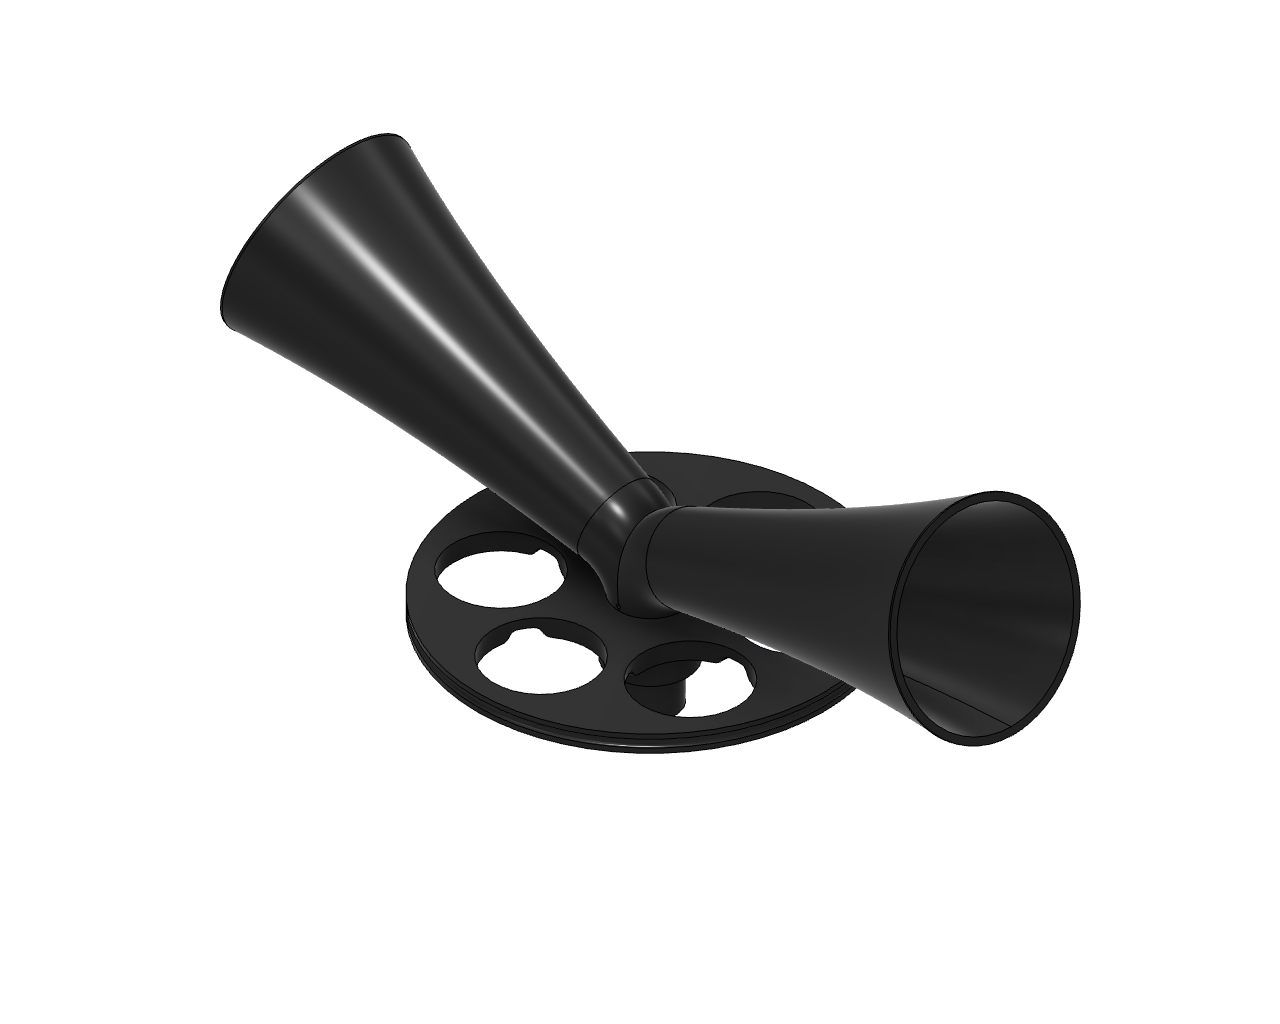
\includegraphics[width=0.48\textwidth]{fig/design/horn-and-pulley-from-above.png}
		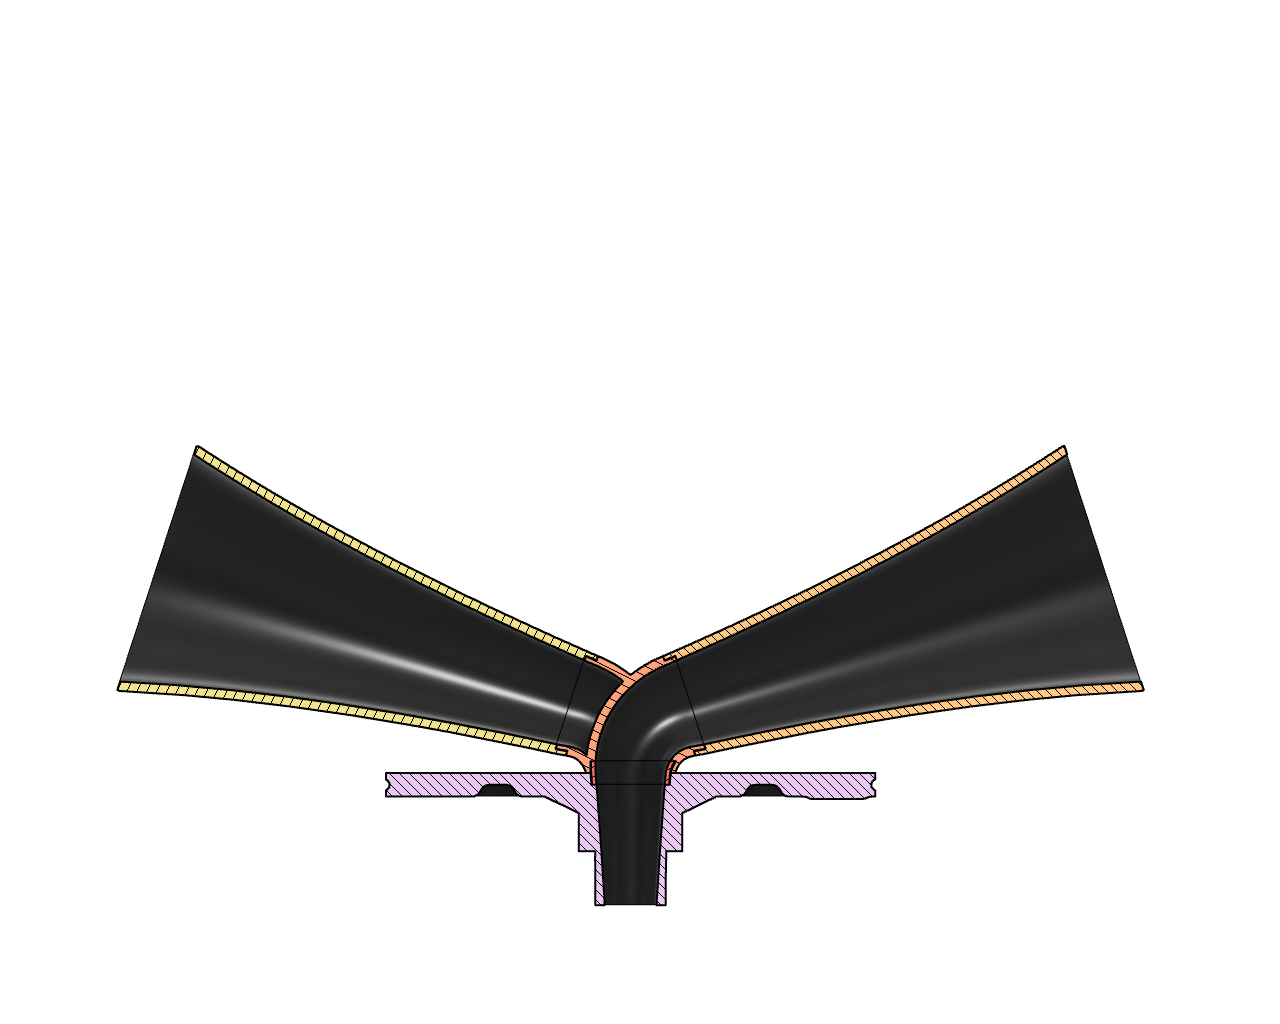
\includegraphics[width=0.48\textwidth]{fig/design/horn-and-pulley.png}
	\end{center}
	\caption{}\label{fig:horn-and-pulley}
\end{figure}

\textbf{TODO: a small thing on one side to place the centre of mass in 0,0}




\subsubsection{Bearing seat and Horn driver mount}


A bearing of type (6306.2zr.c3 kulelager) was bought on Finn.no for 50 kr. A seat to mount the bearing was designed in Autodesk Fusion. A mount for the ma600 encoder was placed according to instructions from \textbf{TODO: blog post fra mj bots}, centred on the magnet 0.5 mm distance.

\begin{figure}[H]
	\begin{center}
		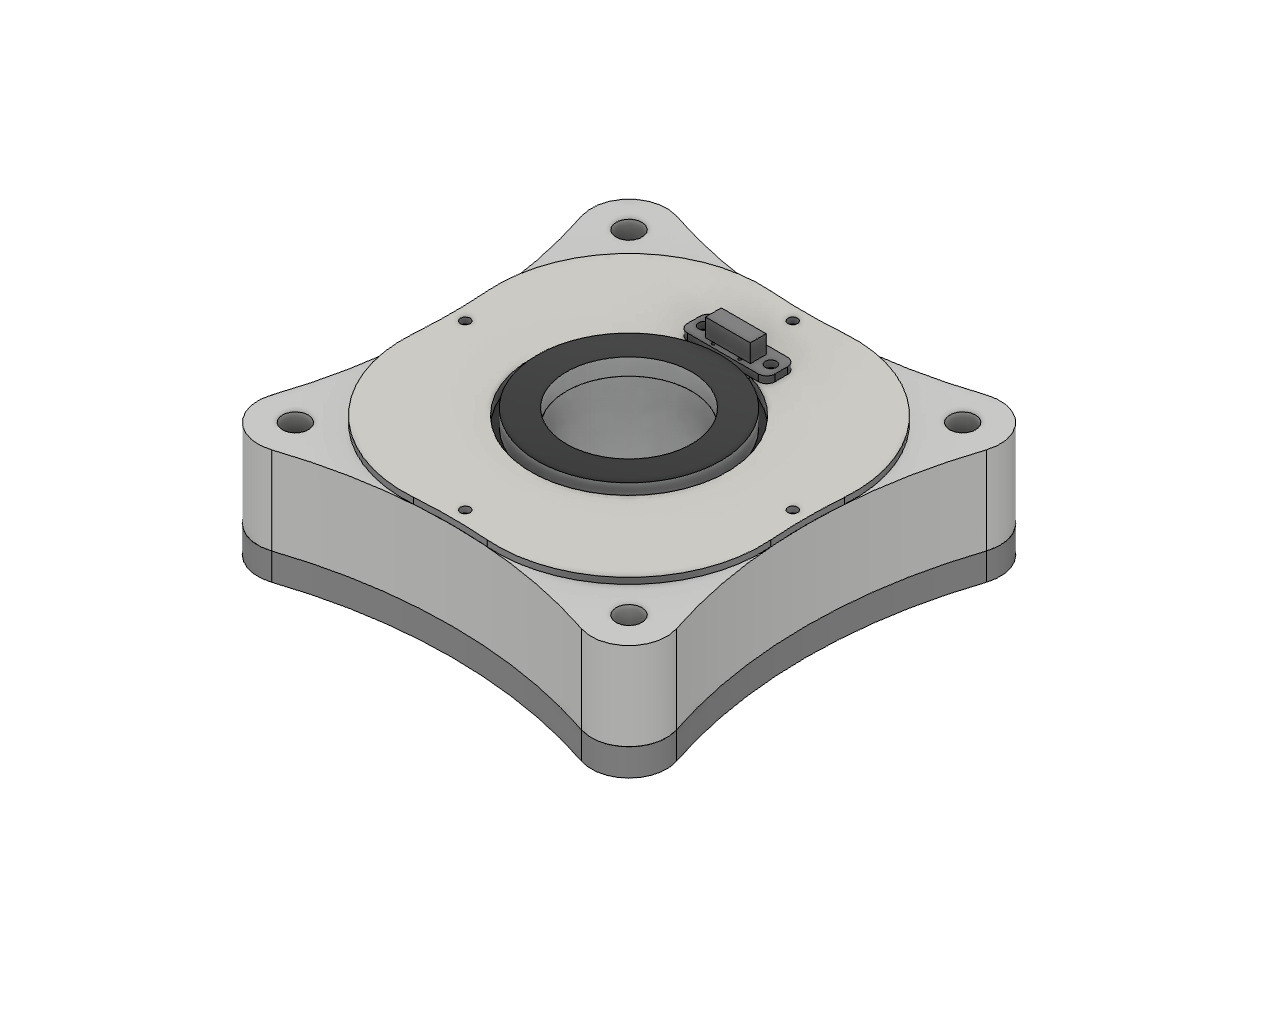
\includegraphics[width=0.48\textwidth]{fig/design/bearing-seat-front.png}
		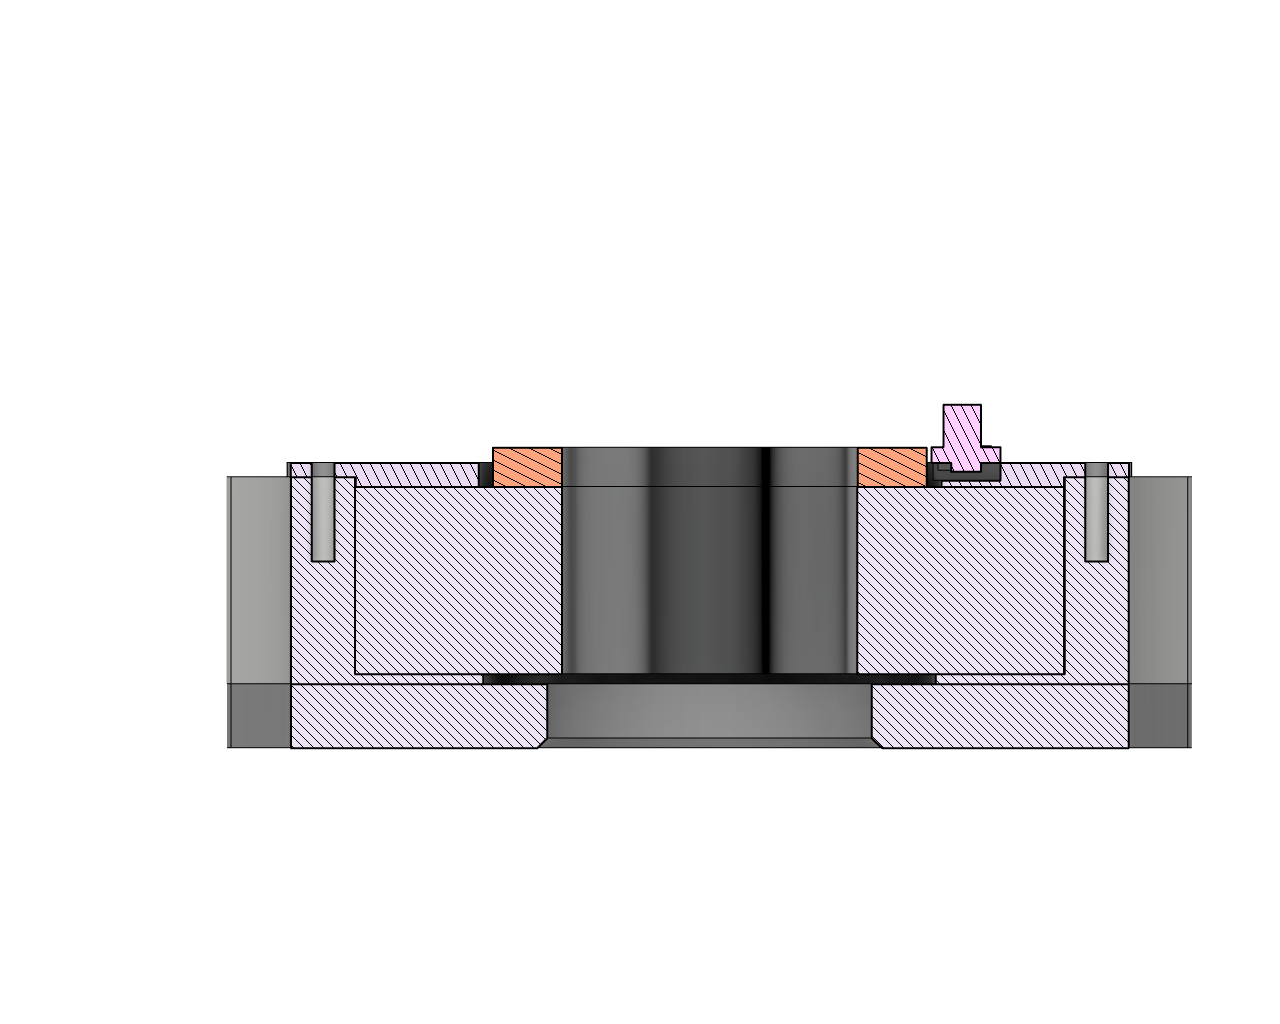
\includegraphics[width=0.48\textwidth]{fig/design/bearing-seat-cross-section.png}
	\end{center}
	\caption{}\label{fig:bearing-seat}
\end{figure}

\begin{figure}[H]
	\begin{center}
		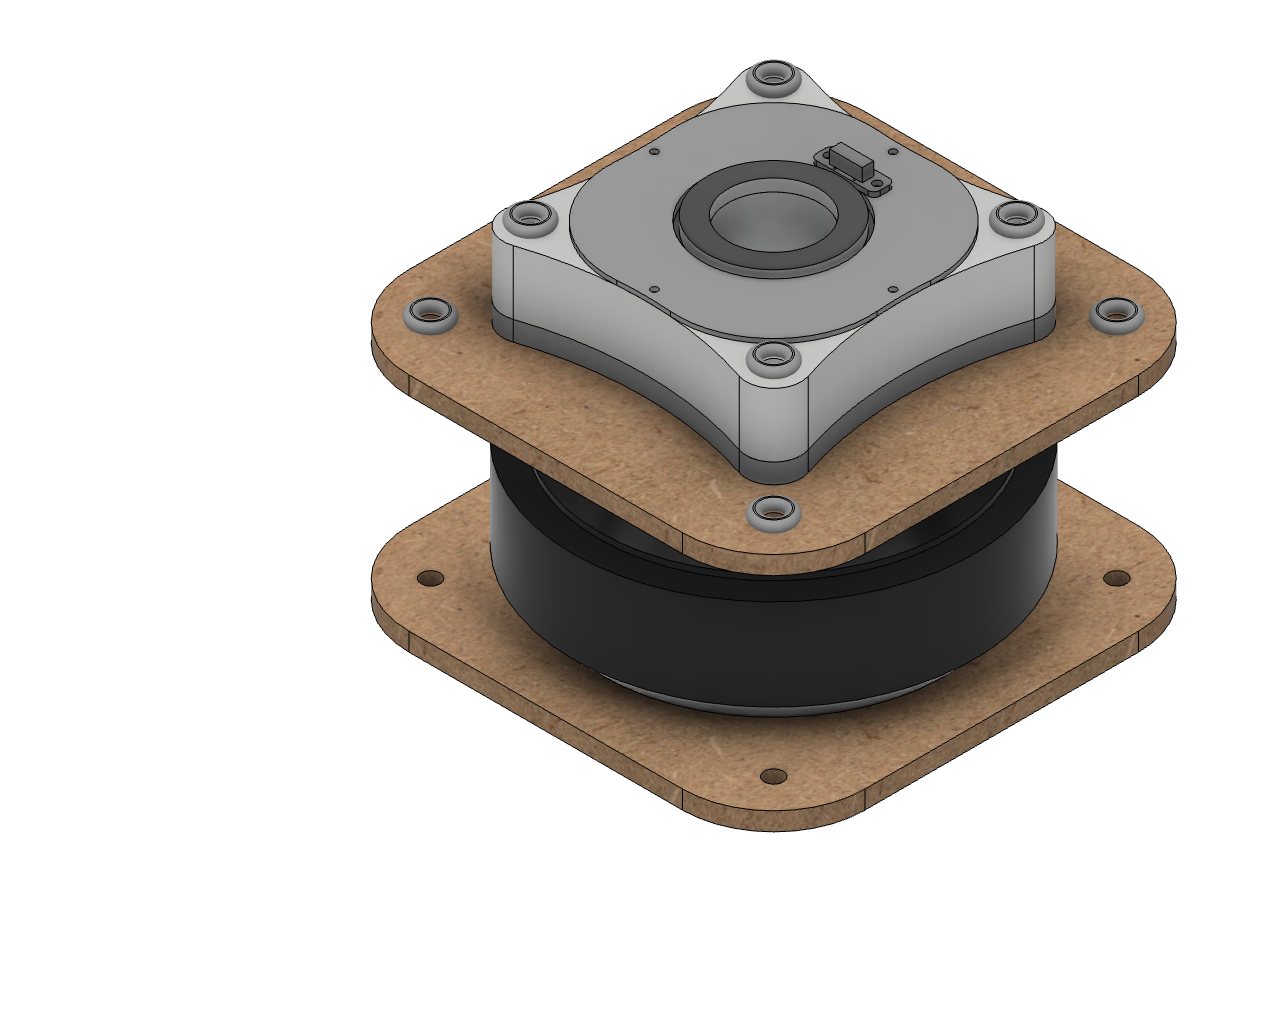
\includegraphics[width=0.48\textwidth]{fig/design/driver and bearing.png}
		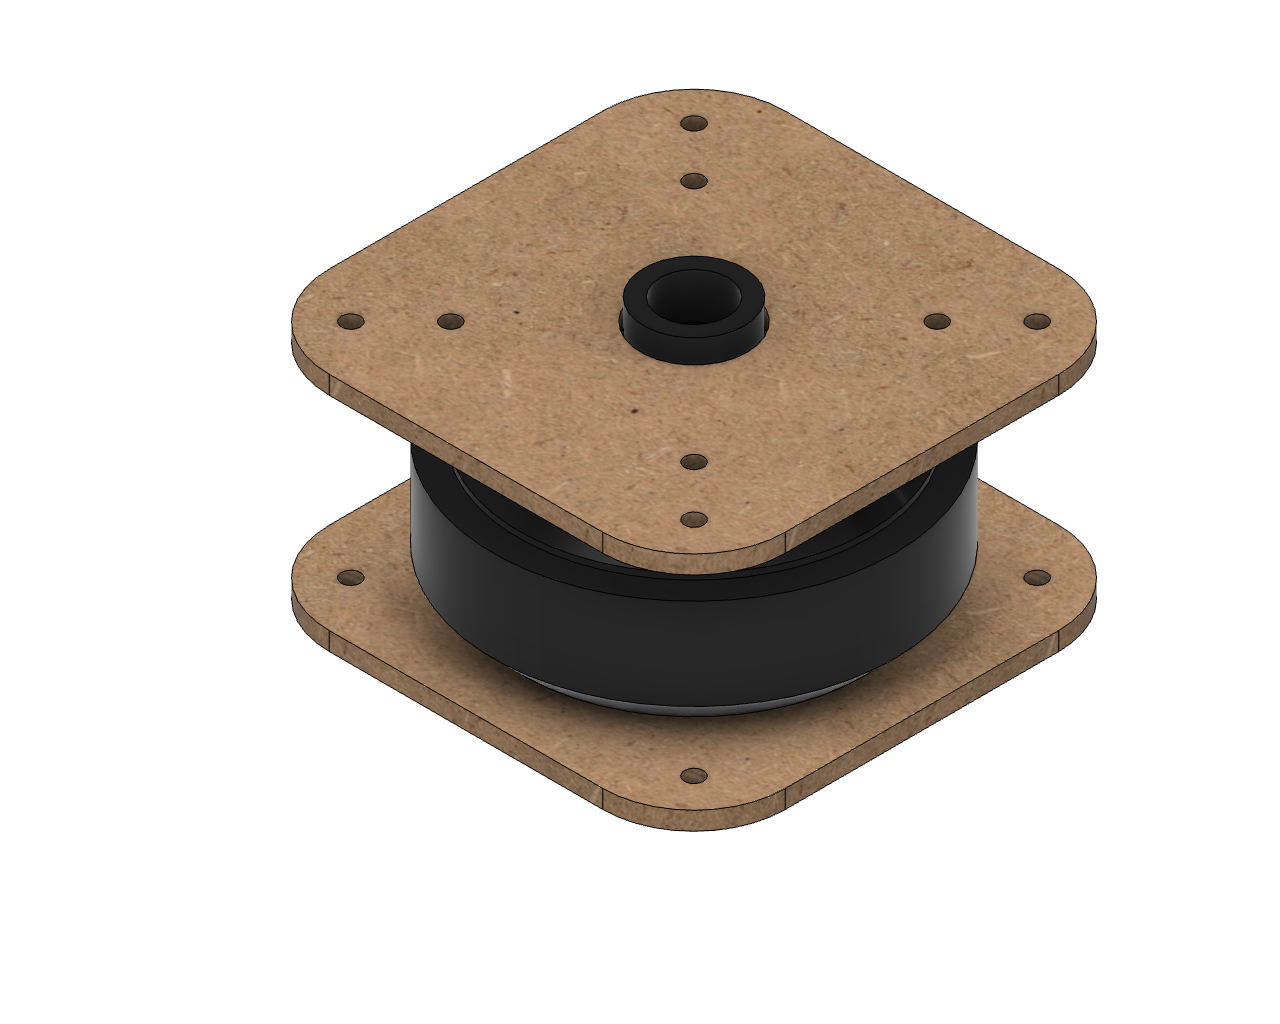
\includegraphics[width=0.48\textwidth]{fig/design/driver.png}
	\end{center}
	\caption{}\label{fig:driver-and-bearing}
\end{figure}

\subsection{Full Horn driver assembly}
\begin{figure}
	\begin{center}
		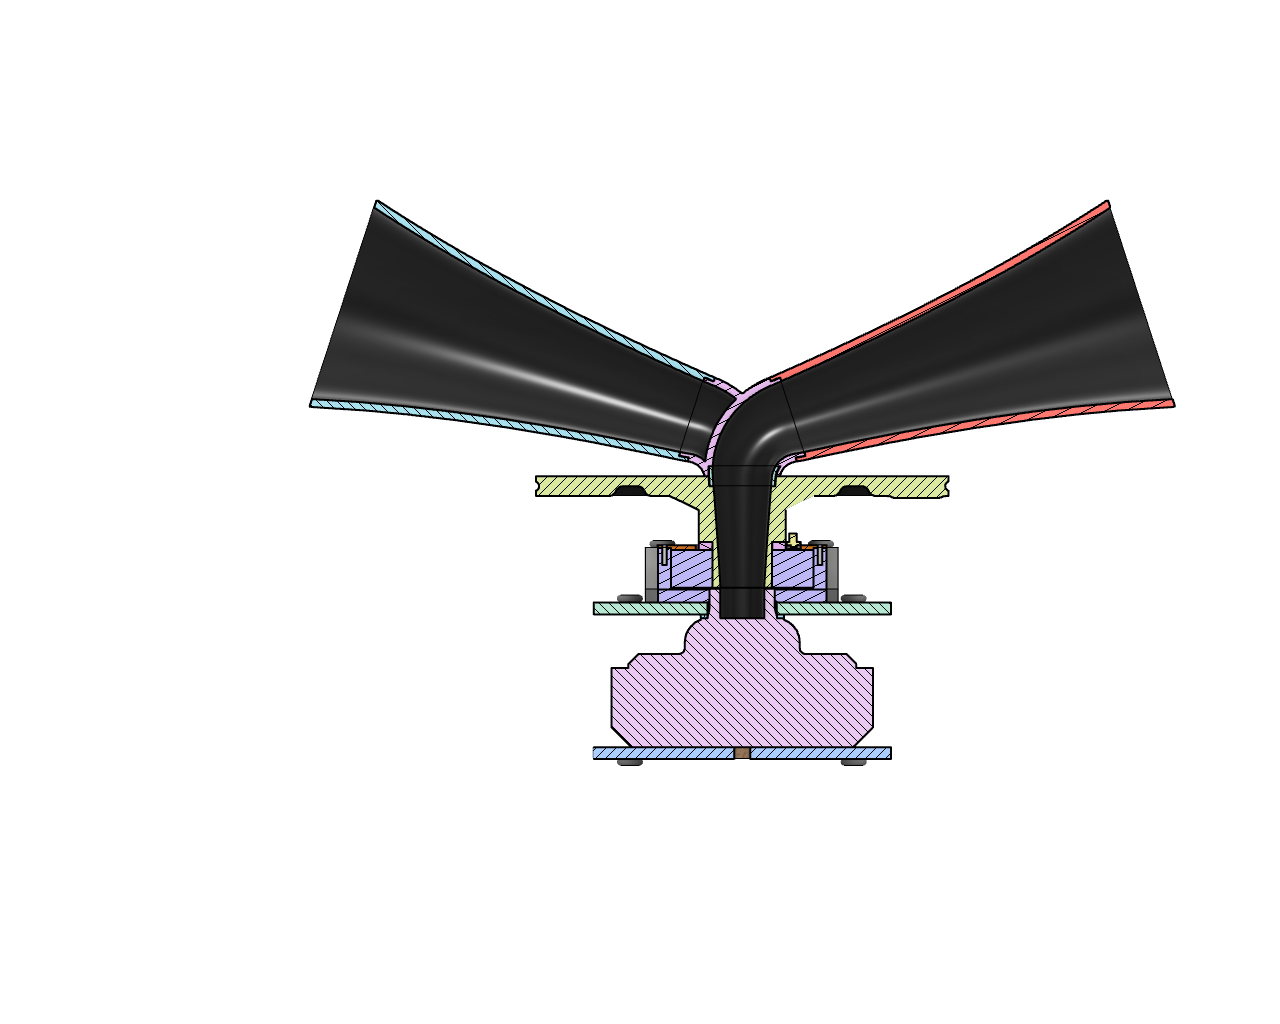
\includegraphics[width=0.95\textwidth]{fig/implementation/horn-driver-assembly.png}
	\end{center}
	\caption{}\label{fig:horn-driver-assembly}
\end{figure}

\subsection{Motor and motor bracket}

The Moteus C1 motor controller uses a diametrically magnetized magnet in order to get feedback for both commutation and position of the rotor shaft. \textbf{TODO: sett inn kilde til moteus dokumentasjon}


"
If using the default onboard encoder, the following steps must be taken:

A diametrically magnetized sense magnet should be attached to the rotor. The fastening must be rigid, allowing no slip. Adhesive is generally required, cyanoacrylate or epoxy can be used.
The moteus controller must be mounted so that the encoder is (a) centered laterally on the sense magnet and (b) has an air-gap of approximately 2mm. This mount must be rigid and allow no slip.
" \citep{mjbots_moteus_mechanical_setup}

In order to mount the Moteus controller precisely in relation to the motor and magnet, a 3D model
of the BLDC motor to be used was designed in Autodesk Fusion, based on the specifications in \autoref{app:motor},


A 3D model of
the Moteus c1 controller circuit board was downloaded from the mj bots website. Then a bracket to
mount the motor controller on the back of the motor was designed in Autodesk Fusion, see \autoref{fig:bracket}
and \autoref{fig:bracket2}


\begin{figure}[H]
	\centering
	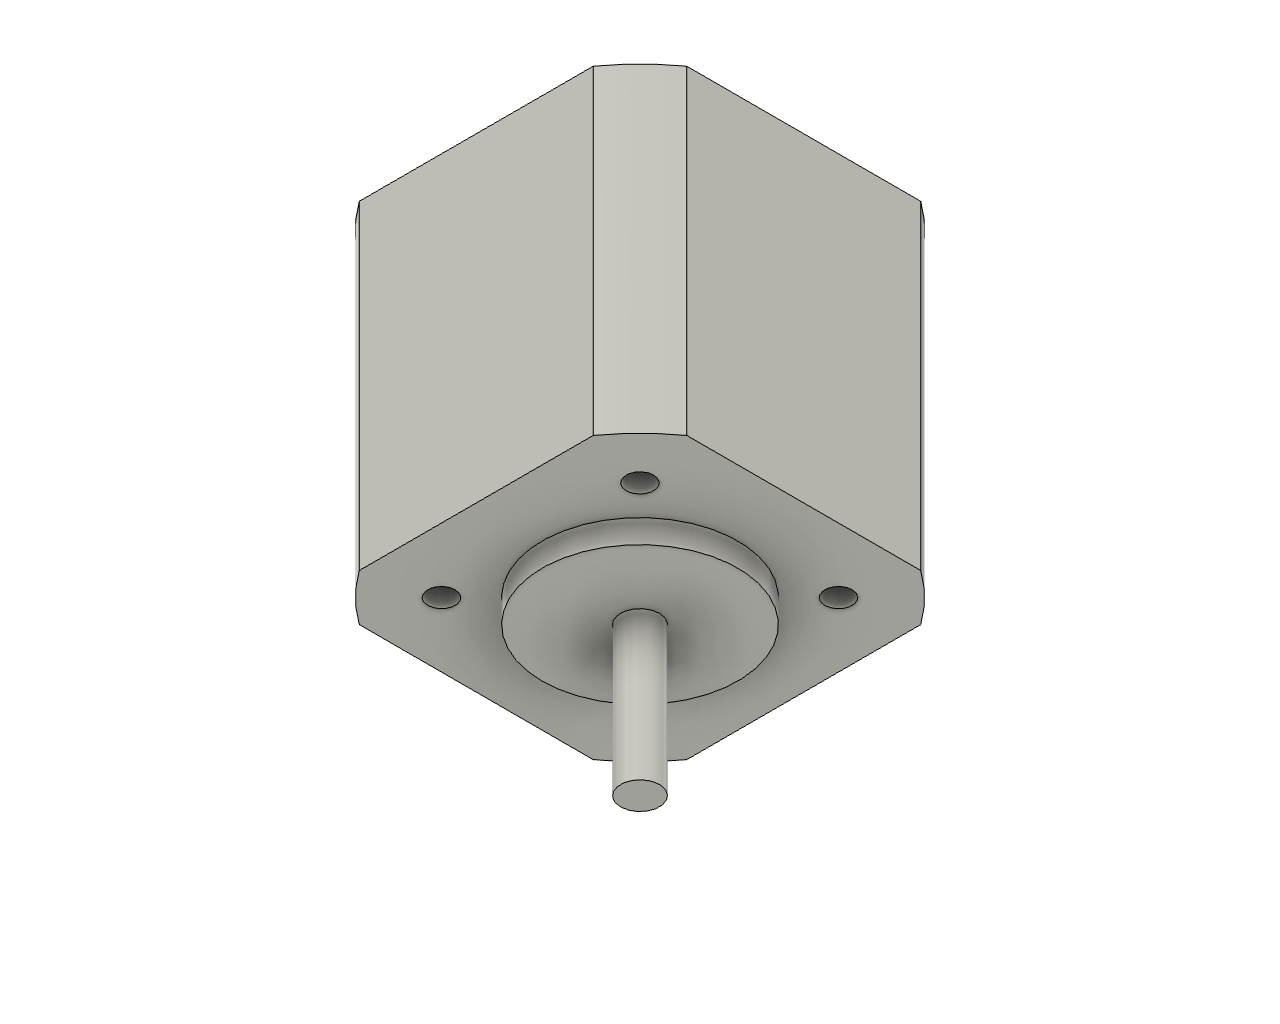
\includegraphics[width=0.48\textwidth]{fig/only-motor.PNG}\hfill
	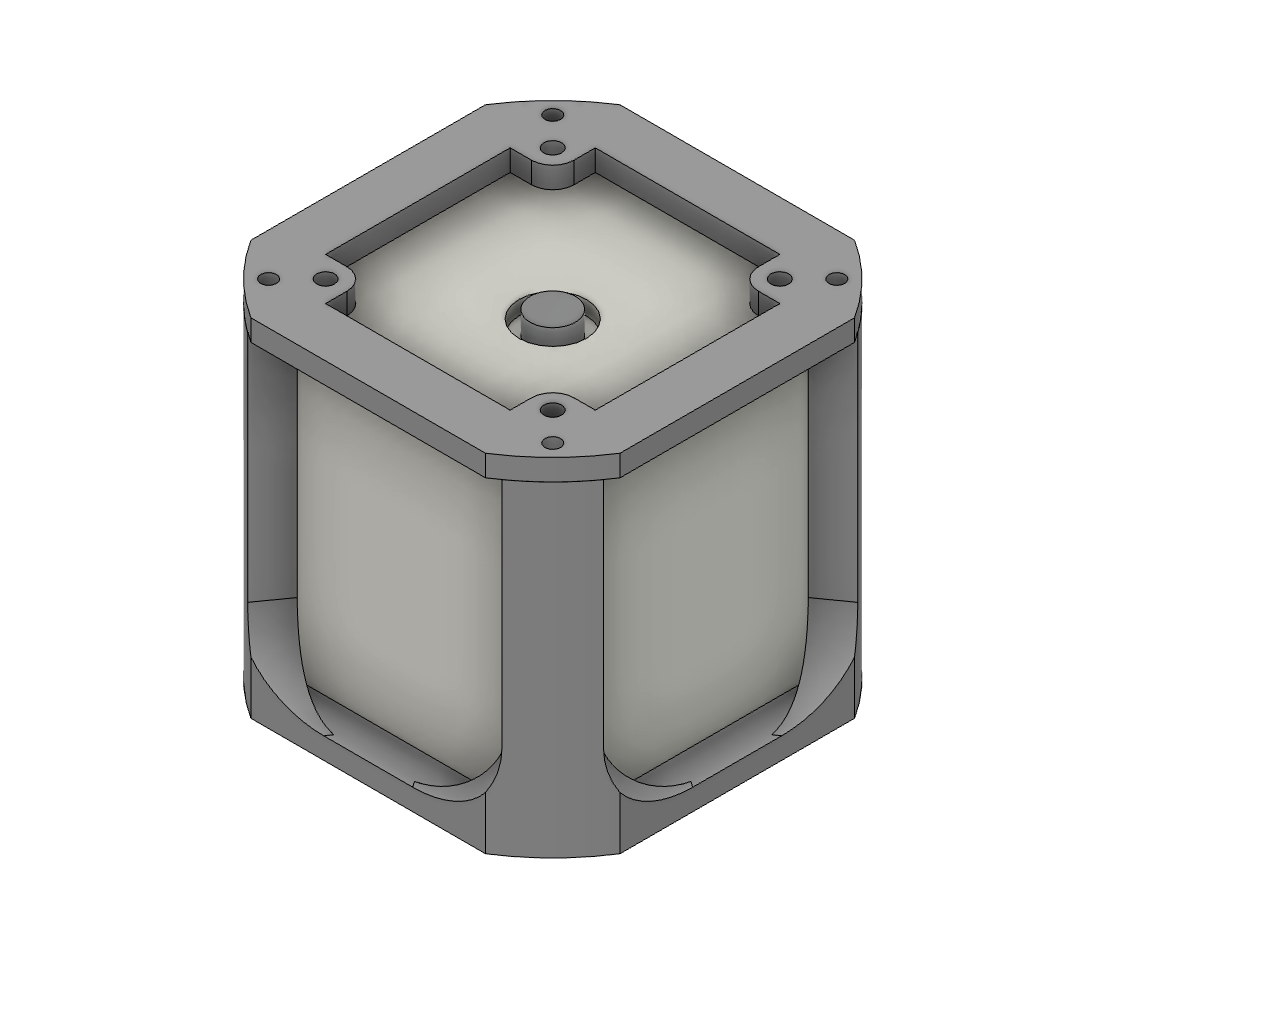
\includegraphics[width=0.48\textwidth]{fig/motor-and-bracket.PNG}\hfill
	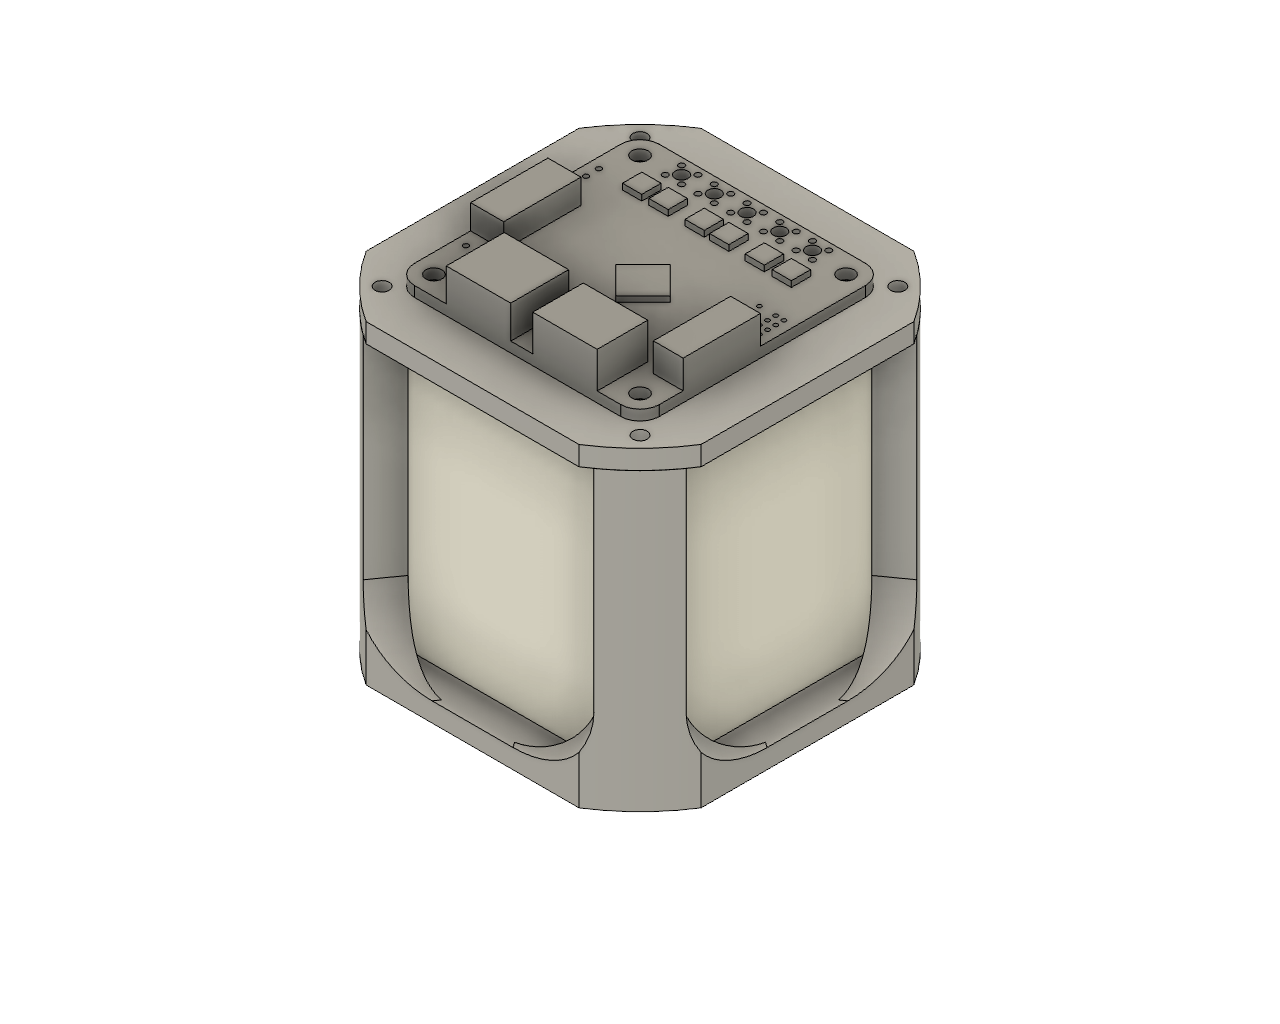
\includegraphics[width=0.48\textwidth]{fig/moteus-motor-bracket-over.PNG}\hfill
	\caption{}
	\label{fig:bracket}
\end{figure}

\begin{figure}[H]
	\centering
	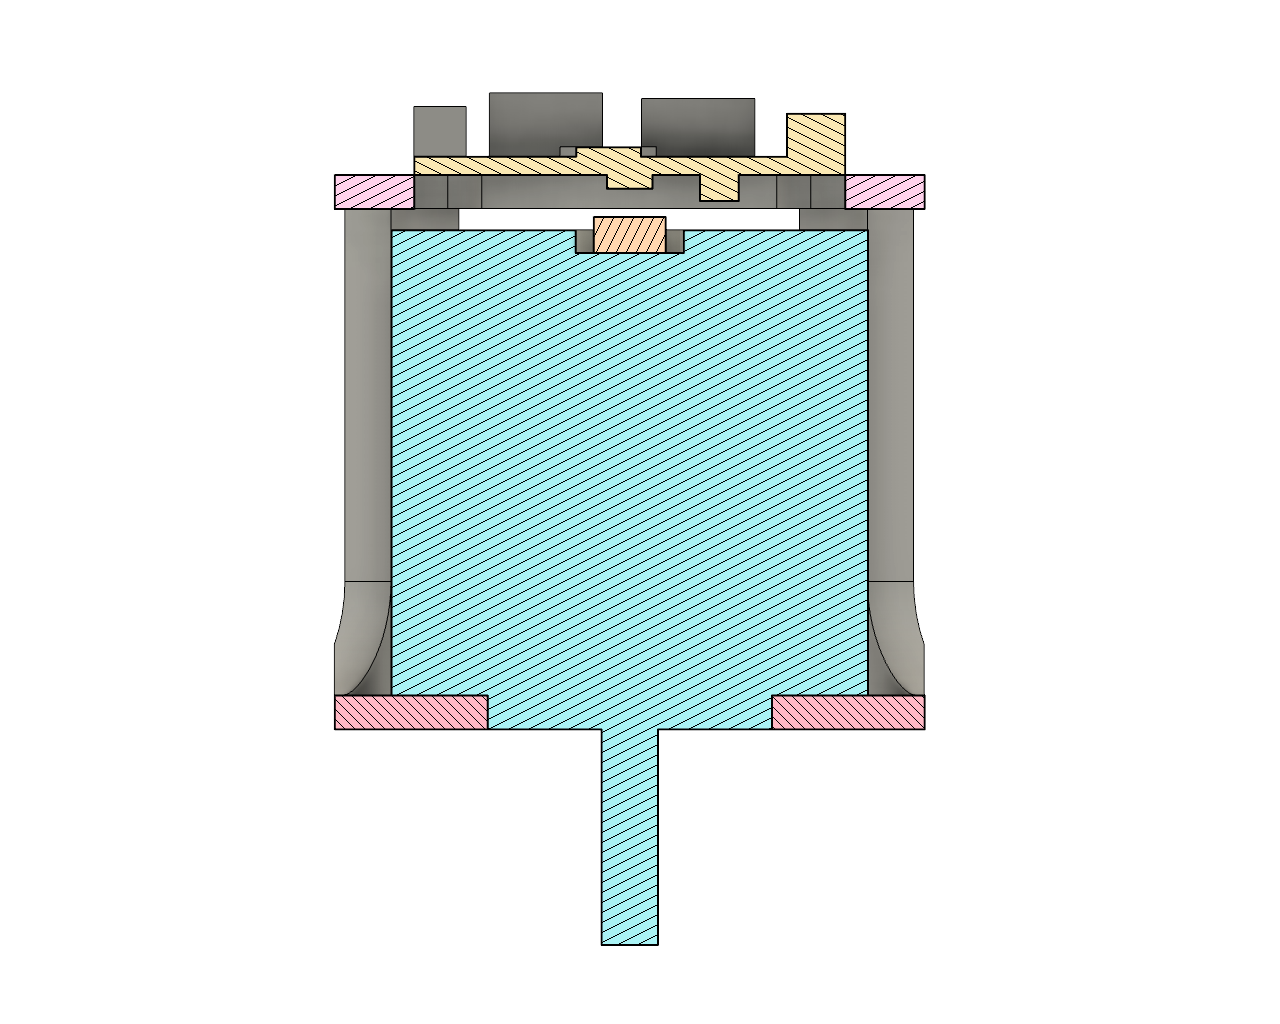
\includegraphics[width=0.8\textwidth]{fig/moteus-motor-bracket-inside.PNG}
	\caption{Motor is blue, motor driver is yellow and magnet is orange.}
	\label{fig:bracket2}
\end{figure}

\subsection{Cabinet design}

According to the manufacturer of the bottom speaker, Celestion, speakers designed for high-fidelity audio or bass cabinets require Thiele-Small parameters to ensure a good result. "Guitar speakers often sound best with a simple, well-constructed, and adequately sized enclosure that focuses on practical dimensions and volume." \textbf{TODO: parafraser}
Celestion states that slight differences in the Thiele-Small parameters will be completely overridden by musical non-linear properties of the guitar speaker especially when driven hard \cite{celestion_1x12_cabinet}.
\textbf{TODO: quote Celestion's website that the Thiele-Small parameters do not matter in a highly non-linear guitar speaker.} Celestion states a recommended internal volume of 42.5 to 70.8 litres as a starting point. According

The internal volume of the cabinet was designed to 49.14 litres. Closed cabinet
\begin{figure}
	\begin{center}
		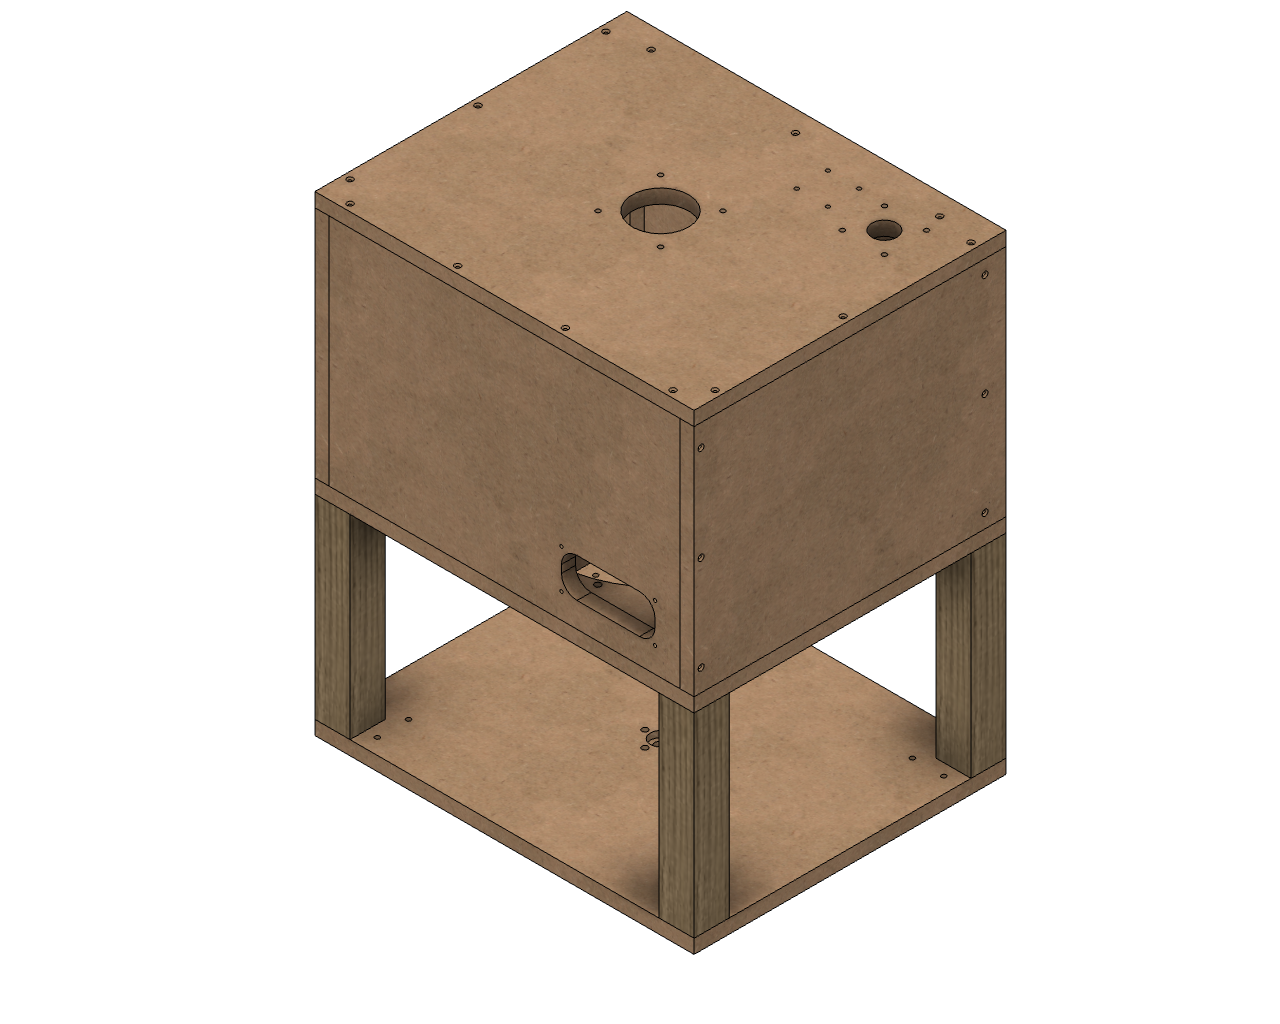
\includegraphics[width=0.48\textwidth]{fig/design/cabinet front.png}\hfill
		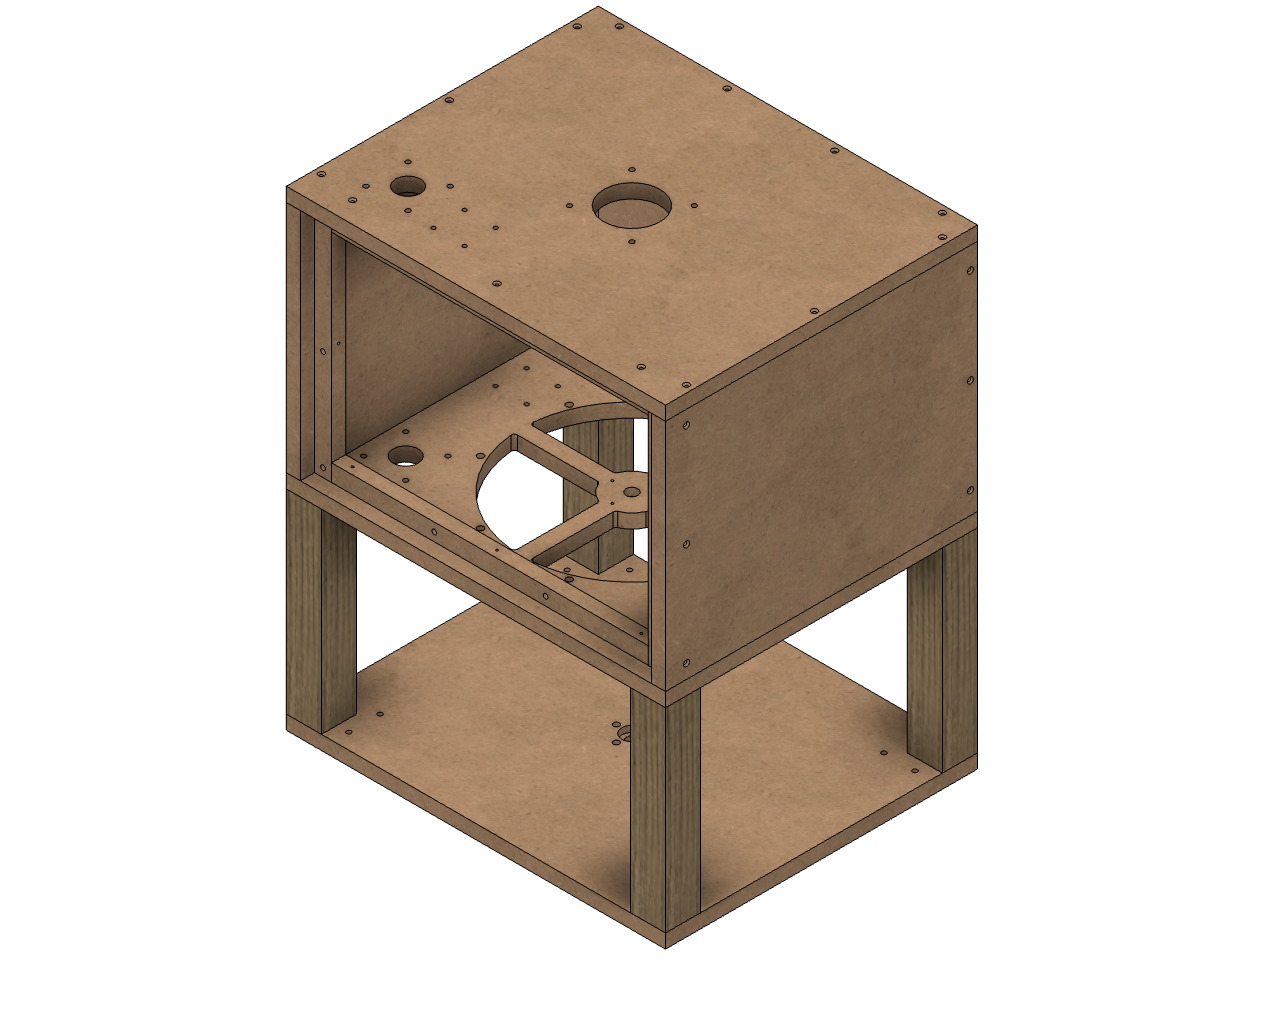
\includegraphics[width=0.48\textwidth]{fig/design/cabinet-back.png}
	\end{center}
	\caption{}\label{fig:cabinet-design}
\end{figure}

\subsection{Piecing everything together}

\newpage
\section{Software}

\section{Controller}
\begin{figure}
	\begin{center}
		% System overview flowchart: DAW → PLL → Position/velocity mapping → Servo system
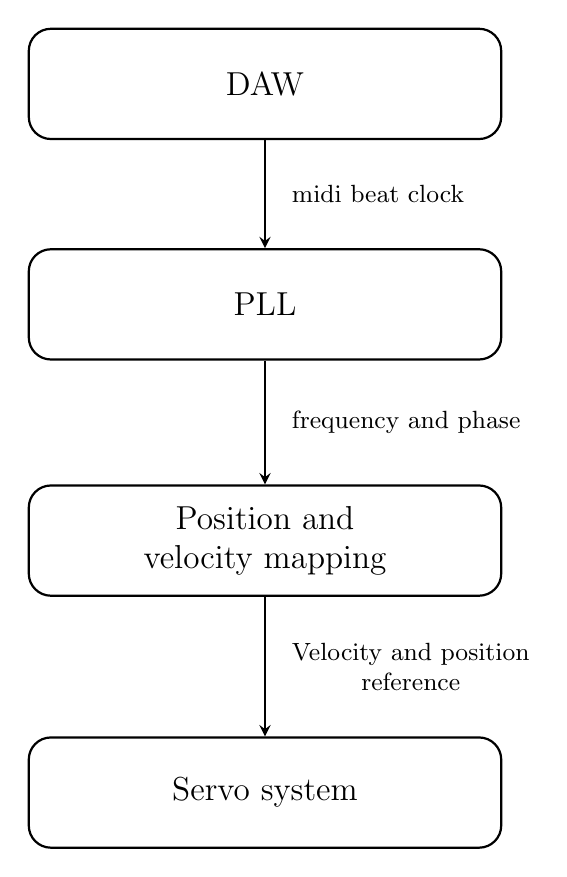
\begin{tikzpicture}[
	box/.style={
		draw, rounded corners=8pt, thick,
		minimum width=6cm, minimum height=1.4cm,
		align=center, font=\large
	},
	arr/.style={->, >=stealth, thick},
	lbl/.style={font=\small, align=center}
]

\node[box] (daw)     at (0,  0)   {DAW};
\node[box] (pll)     at (0, -2.8) {PLL};
\node[box] (mapping) at (0, -5.8) {Position and\\velocity mapping};
\node[box] (servo)   at (0, -9.0) {Servo system};

\draw[arr] (daw.south)     -- node[lbl, right=6pt] {midi beat clock}              (pll.north);
\draw[arr] (pll.south)     -- node[lbl, right=6pt] {frequency and phase}          (mapping.north);
\draw[arr] (mapping.south) -- node[lbl, right=6pt] {Velocity and position\\reference} (servo.north);

\end{tikzpicture}

	\end{center}
	\caption{}\label{fig:system-overview}
\end{figure}

\subsection{Control Laws}


\begin{figure}
	\begin{center}
		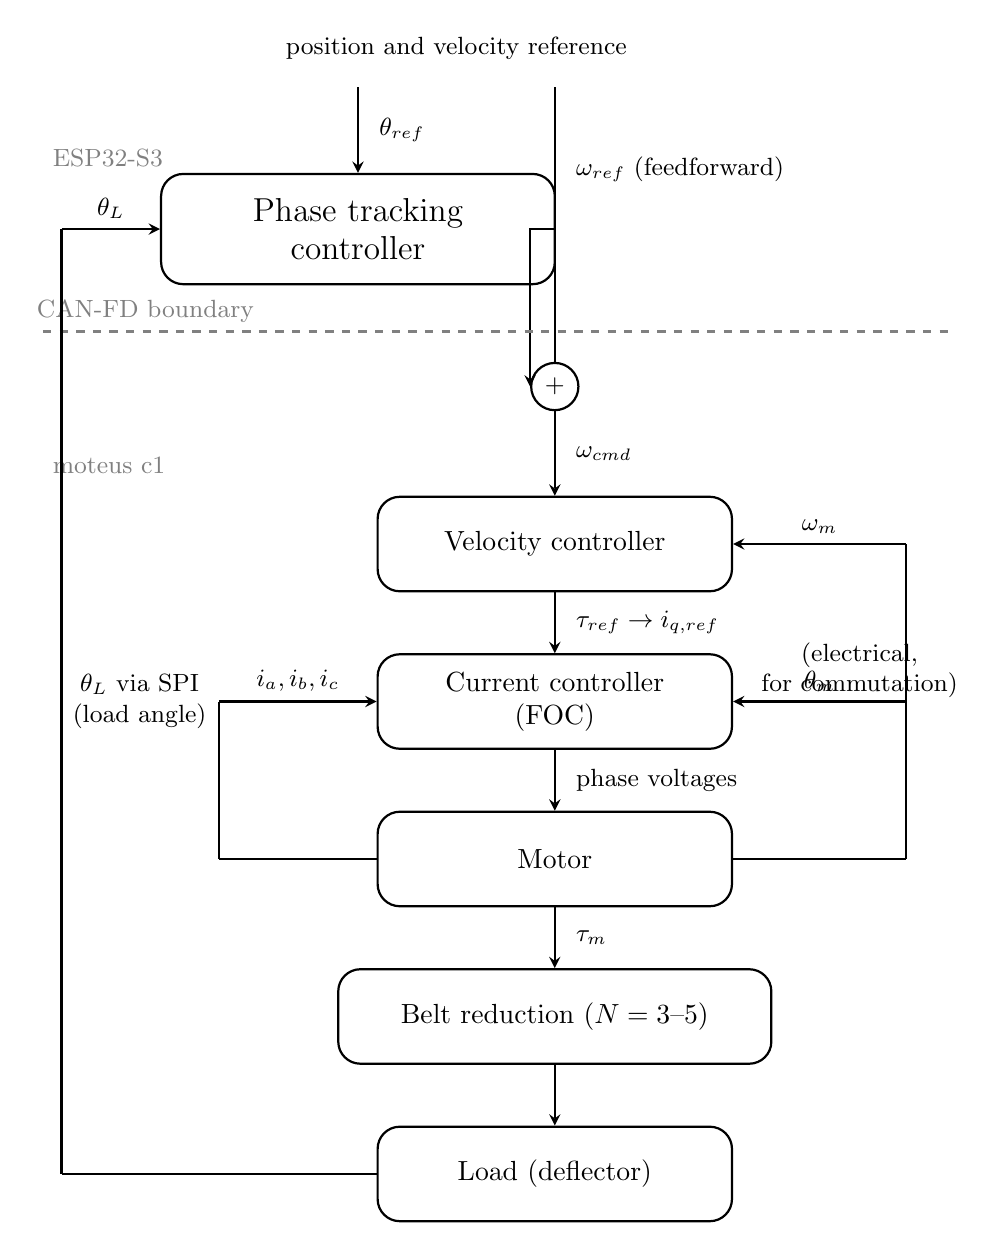
\begin{tikzpicture}[
		box/.style={
				draw, rounded corners=8pt, thick,
				minimum width=5cm, minimum height=1.4cm,
				align=center, font=\large
			},
		smallbox/.style={
				draw, rounded corners=8pt, thick,
				minimum width=4.5cm, minimum height=1.2cm,
				align=center, font=\normalsize
			},
		container/.style={
				draw, rounded corners=10pt, thick, dashed,
				inner sep=10pt
			},
		sum/.style={
				draw, circle, thick, inner sep=1pt,
				minimum size=6mm, font=\small
			},
		arr/.style={->, >=stealth, thick},
		line/.style={thick},
		lbl/.style={font=\small, align=center},
		boundary/.style={dashed, thick, gray}
	]

	% Phase tracking controller
	\node[box] (ptc) at (0, 0) {Phase tracking\\controller};

	% Summing junction
	\node[sum] (sum) at (2.5, -2.0) {$+$};

	% Velocity controller
	\node[smallbox] (vel) at (2.5, -4.0) {Velocity controller};

	% Current controller
	\node[smallbox] (cur) at (2.5, -6.0) {Current controller\\(FOC)};

	% Motor
	\node[smallbox] (motor) at (2.5, -8.0) {Motor};

	% Belt reduction
	\node[smallbox, minimum width=5.5cm] (belt) at (2.5, -10.0) {Belt reduction ($N=3\text{–}5$)};

	% Load
	\node[smallbox] (load) at (2.5, -12.0) {Load (deflector)};

	% Reference inputs (top)
	\coordinate (refin)  at (0,  1.8);
	\coordinate (ffin)   at (2.5, 1.8);

	\draw[arr] (refin) -- node[lbl, right=4pt, pos=0.5] {$\theta_\text{ref}$} (ptc.north);
	\draw[line] (ffin) -- node[lbl, right=4pt, pos=0.3] {$\omega_\text{ref}$ (feedforward)} (sum.north);

	% Common input label above
	\node[lbl] at (1.25, 2.3) {position and velocity reference};

	% PTC -> sum
	\draw[arr] (ptc.east) -| (sum.west);

	% sum -> velocity controller
	\draw[arr] (sum.south) -- node[lbl, right=4pt] {$\omega_\text{cmd}$} (vel.north);

	% velocity -> current
	\draw[arr] (vel.south) -- node[lbl, right=4pt] {$\tau_\text{ref} \to i_{q,\text{ref}}$} (cur.north);

	% current -> motor
	\draw[arr] (cur.south) -- node[lbl, right=4pt] {phase voltages} (motor.north);

	% motor -> belt
	\draw[arr] (motor.south) -- node[lbl, right=4pt] {$\tau_m$} (belt.north);

	% belt -> load
	\draw[arr] (belt.south) -- (load.north);

	% CAN-FD boundary line
	\draw[boundary] (-4.0, -1.3) -- (7.5, -1.3);
	\node[lbl, gray] at (-2.7, -1.05) {CAN-FD boundary};

	% ESP32 label
	\node[lbl, gray, anchor=west] at (-4.0, 0.9) {ESP32-S3};

	% moteus label
	\node[lbl, gray, anchor=west] at (-4.0, -3.0) {moteus c1};

	% Feedback: motor -> velocity controller (omega_m)
	\draw[line] (motor.east) -- ++(2.2, 0) coordinate (fb1);
	\draw[line] (fb1) -- (fb1 |- vel.east);
	\draw[arr]  (fb1 |- vel.east) -- node[lbl, above, pos=0.5] {$\omega_m$} (vel.east);

	% Feedback: motor -> current controller (theta_m for commutation)
	\draw[line] (motor.east) ++(2.2, 0) -- ++(0, 2.0) coordinate (fb2);
	\draw[line] (fb2) -- (fb2 |- cur.east);
	\draw[arr]  (fb2 |- cur.east) -- node[lbl, above, pos=0.5] {$\theta_m$} (cur.east);
	\node[lbl, anchor=west] at (5.0, -5.6) {(electrical,\\for commutation)};

	% Feedback: phase currents -> current controller
	\draw[line] (motor.west) -- ++(-2.0, 0) coordinate (fbc);
	\draw[line] (fbc) -- (fbc |- cur.west);
	\draw[arr]  (fbc |- cur.west) -- node[lbl, above, pos=0.5] {$i_a, i_b, i_c$} (cur.west);

	% Feedback: load -> phase tracking controller (theta_L)
	\draw[line] (load.west) -- ++(-4.0, 0) coordinate (fbl);
	\draw[line] (fbl) -- (fbl |- ptc.west);
	\draw[arr]  (fbl |- ptc.west) -- node[lbl, above, pos=0.5] {$\theta_L$} (ptc.west);
	\node[lbl, anchor=east] at (-1.8, -6.0) {$\theta_L$ via SPI\\(load angle)};

\end{tikzpicture}

	\end{center}
	\caption{}\label{fig:servo-system}
\end{figure}


\cleardoublepage
